% ===== CHAPTER 5 =====
\chapter{角动量}
\label{chap:5}
\section{同时确定多个属性}
\label{sec:5.1 Simultaneous Specification of Several Properties}
    在本章中,我们将讨论角动量,在下一章中,我们将证明对于氢原子的静止态,电子角动量的大小是恒定的。首先,我们要考虑用什么标准来决定一个系统的哪些性质可以同时赋予定值。

    在第\ref{sec:3.3 Operators and Quantum Mechanics}节中,我们假设:若态函数$\Psi$时算符$\hat{A}$的本征函数,本征值为$s$,则对物理量$A$的测量结果一定为为$s$。若$\Psi$同时是$\hat{A}$和$\hat{B}$的本征函数,即$\hat{A}\Psi=s\Psi$,$\hat{B}\Psi=t\Psi$,那么我们就可以同时为物理量 $A$ 和 $B$ 赋以确定的值。什么时候$\Psi$会同时是两个算符的本征函数呢?在第\ref{chap:7}章中,我们将证明如下两个理论。首先,两个算符的同时本征函数的完整集合存在的必要条件是算符之间可对易(这里使用的“\textit{完整}”一词有一定的技术含义,我们将在第 \ref{chap:7} 章再讨论这个问题)。反之亦然,若对应于物理量的两个算符$\hat{A}$ 和 $\hat{B}$ 可对易,则存在一组完整的函数,它们同时是$\hat{A}$和$\hat{B}$的本征函数。因此,若$\left[\hat{A},\hat{B}\right]=0$,那么$\Psi$可以同时是$\hat{A}$和$\hat{B}$的本征函数。

    回忆算符$\hat{A}$和$\hat{B}$的交换子为$\left[\hat{A},\hat{B}\right] \equiv \hat{A}\hat{B} - \hat{B}\hat{A}$[式(\ref{eq:3.7 definition of commutator for two operators})]。下列等式有助于计算交换子。通过详细写出交换子可以证明这些等式(问题5.2):
    \begin{equation}
        \boxed{
            \left[\hat{A},\hat{B}\right] = -\left[\hat{B},\hat{A}\right]
        }
        \label{eq:5.1}
    \end{equation}
    \begin{equation}
        \boxed{
            \left[\hat{A}, \hat{A}^n\right] = 0, \quad n = 1, 2, 3, \ldots
        }
        \label{eq:5.2}
    \end{equation}
    \begin{equation}
        \boxed{
            \left[k\hat{A},\hat{B}\right] = \left[\hat{A}, k\hat{B}\right] = k\left[\hat{A},\hat{B}\right]
        }
        \label{eq:5.3}
    \end{equation}
    \begin{equation}
        \boxed{
            \left[\hat{A}, \hat{B}+\hat{C}\right] = \left[\hat{A},\hat{B}\right] + \left[\hat{A},\hat{C}\right]
        }
        \quad 
        \boxed{
            \left[\hat{A}+\hat{B},\hat{C}\right] = \left[\hat{A},\hat{C}\right] + \left[\hat{B},\hat{C}\right]
        }
        \label{eq:5.4}
    \end{equation}
    \begin{equation}
        \boxed{
            \left[\hat{A}, \hat{B}\hat{C}\right] = \left[\hat{A},\hat{B}\right]\hat{C} + \hat{B}\left[\hat{A},\hat{C}\right]
        }
        \quad
        \boxed{
            \left[\hat{A}\hat{B},\hat{C}\right] = \hat{A}\left[\hat{B},\hat{C}\right] + \left[\hat{A},\hat{C}\right]\hat{B}
        }
        \label{eq:5.5}
    \end{equation}
    其中$k$是常数,所有算符都假设为线性算符。
    \begin{examplebox}
        \textbf{例题:}从$\left[\partial/\partial x,x\right]=1$[式(\ref{eq:3.8})]出发,使用对易子的性质(式(\ref{eq:5.1})至(\ref{eq:5.5}))求以下对易子:(a)$\left[\hat{x},\hat{p_x}\right]$;(b)$\left[\hat{x}, \hat{p_x^2}\right]$;(c)三维单粒子系统的$\left[\hat{x},\hat{H}\right]$。
        \\
        (a)使用式(\ref{eq:5.3})和(\ref{eq:5.1}),因为$\left[\partial/\partial x,x\right]=1$,我们有
        \begin{equation*}
            \left[\hat{x},\hat{p_x}\right] = \left[\hat{x},\frac{\hbar}{\mathrm{i}}\frac{\partial}{\partial x}\right] = \frac{\hbar}{\mathrm{i}}\left[\hat{x},\frac{\partial}{\partial x}\right] = -\frac{\hbar}{\mathrm{i}}\left[\frac{\partial}{\partial x},\hat{x}\right] = -\frac{\hbar}{\mathrm{i}}
        \end{equation*}
        \begin{equation}
            \left[\hat{x},\hat{p_x}\right]=\mathrm{i}\hbar
            \label{eq:5.6}
        \end{equation}
        (b)由式(\ref{eq:5.5})和(\ref{eq:5.6}),有
        \begin{equation*}
            \left[\hat{x},\hat{p_x^2}\right] = \left[\hat{x},\hat{p_x}\right]\hat{p_x} + \hat{p_x}\left[\hat{x},\hat{p_x}\right] = \mathrm{i}\hbar\cdot\frac{\hbar}{\mathrm{i}}\frac{\partial}{\partial x} + \frac{\hbar}{\mathrm{i}}\frac{\partial}{\partial x} \cdot \mathrm{i}\hbar
        \end{equation*}
        \begin{equation}
            \left[\hat{x},\hat{p_x^2}\right] = 2\hbar^2\frac{\partial}{\partial x}
            \label{eq:5.7}
        \end{equation}
        (c)使用式(\ref{eq:5.4})、(\ref{eq:5.3})和(\ref{eq:5.7}),有
        \begin{equation*}
            \begin{aligned}
                \left[\hat{x},\hat{H}\right] &= \left[\hat{x},\hat{T}+\hat{V}\right] = \left[\hat{x},\hat{T}\right] + \left[\hat{x},\hat{V}\left(x,y,z\right)\right] =\left[\hat{x},\hat{T}\right] \\
                &= \left[\hat{x}, \left(1/2m\right)\left(\hat{p_x^2}+\hat{p_y^2}+\hat{p_z^2}\right)\right]\\
                &= \left(1/2m\right)\left[\hat{x},\hat{p_x^2}\right] + \left(1/2m\right)\left[\hat{x},\hat{p_y^2}\right] + \left(1/2m\right)\left[\hat{x},\hat{p_z^2}\right]\\
                &= \frac{1}{2m}2\hbar^2\frac{\partial}{\partial x} + 0 + 0
            \end{aligned}
        \end{equation*}
        \begin{equation}
            \left[\hat{x},\hat{H}\right] = \frac{\hbar^2}{m}\frac{\partial}{\partial x} = \frac{\mathrm{i}\hbar}{m}\hat{p_x}
            \label{eq:5.8}
        \end{equation}
        \\
        \textbf{练习:}求证:对于单粒子三维系统,有
        \begin{equation}
            \left[\hat{p_x^2},\hat{H}\right] = -\mathrm{i}\hbar \:\partial V\left(x,y,z\right)/\partial x
            \label{eq:5.9}
        \end{equation}
    \end{examplebox}

    这些对易子有重要的物理影响。由于$\left[\hat{x},\hat{p_x}\right] \neq 0$,我们不能希望态函数同时是$\hat{x}$和$\hat{p_x}$的本征函数。因此,与不确定性原理相符,我们不能同时测定$x$和$p_x$的精确值。由于$\hat{x}$与$\hat{H}$不可对易,我们不能指望同时为能量和 $x$ 坐标赋予确定的值。定态(具有确定的能量)会显示出$x$的各种可能值,观察到各种$x$值的概率由玻恩公设给出。

    对于不是$\hat{A}$的本征函数的态函数$\Psi$,在完全相同的系统中对$A$的测量将得到各种可能的结果。我们需要对观测值 $A_i$ 的分布或离散性进行某种测量。如果 $\langle A \rangle$ 是这些值的平均值,那么每个测量值与平均值的偏差为$A_i - \langle A \rangle$。如果我们对所有偏差求平均值,就会得到零,因为正负偏差会抵消。因此,为了使所有偏差都为正值,我们要将它们平方。偏差平方的平均值称为 $A$ 的\textbf{方差}(variance),在统计学中用 $\sigma^2\left(A\right)$ 表示,在量子力学中用 $\left(\Delta A\right)^2$ 表示:
    \begin{equation}
        \left(\Delta A\right)^2 \equiv \sigma^2\left(A\right) = \langle \left(A - \langle A \rangle\right)^2 \rangle = \int \Psi^{\ast}\left(\hat{A}-\langle A \rangle\right)^2\Psi\mathrm{d}\tau
        \label{eq:5.10}
    \end{equation}
    其中我们用到了平均值的表达式(\ref{eq:3.88})。定义(\ref{eq:5.10})与以下表达式等价(问题5.7):
    \begin{equation}
        \left(\Delta A\right)^2 = \langle A^2 \rangle - \langle A \rangle^2
        \label{eq:5.11}
    \end{equation}

    方差的正平方根称为\textbf{标准差}(standard deviation),用 $\Delta A$ 或$\sigma\left(A\right)$ 表示。标准差是最常用的价差度量,我们将用它来度量属性 $A$ 的 “不确定性”。

    罗伯逊(Robertson)于 1929 年证明,状态函数为 $\Psi$ 的量子力学系统的两个属性的标准偏差的乘积必须满足不等式
    \begin{equation}
        \sigma\left(A\right)\sigma\left(B\right) = \Delta A \Delta B \ge \frac{1}{2}\left|\int \Psi^{\ast}\left[\hat{A},\hat{B}\right]\Psi\mathrm{d}\tau\right|
        \label{eq:5.12}
    \end{equation}
    (\ref{eq:5.12}) 的证明源于量子力学公设,见问题 7.60。如果$\hat{A}$和$\hat{B}$可对易,那么式(\ref{eq:5.12})中的积分为零,则$\Delta A$和$\Delta B$可能都为零,与上文的讨论相符。

    作为式(\ref{eq:5.12})的一个例子,我们使用式(\ref{eq:5.6})、$\left|z_1z_2\right|=\left|z_1\right|\left|z_2\right|$[式(\ref{eq:1.34 properties of product and quotient absolute values})],以及归一化方法:
    \begin{equation*}
        \Delta x \Delta p_x \ge \frac{1}{2}\left|\int \Psi^{\ast}\left[\hat{x},\hat{p_x}\right]\Psi\mathrm{d}\tau\right| = \frac{1}{2}\left|\int \Psi^{\ast}\mathrm{i}\hbar\Psi\mathrm{d}\tau\right| = \frac{1}{2}\hbar\left|\mathrm{i}\right|\left|\int \Psi^{\ast}\Psi\mathrm{d}\tau\right|
    \end{equation*}
    \begin{equation}
        \sigma\left(x\right)\sigma\left(p_x\right) \equiv \Delta x \Delta p_x \ge \frac{1}{2}\hbar
        \label{eq:5.13}
    \end{equation}

    式(\ref{eq:5.13})通常被认为是\textbf{海森堡不确定性原理}(Heisenberg Uncertainty Principle)(第\ref{sec:1.3 The Uncertainty Principle}节)的定量表述。然而,公式 (\ref{eq:5.12}) 和 (\ref{eq:5.13}) 中标准偏差的含义与第 \ref{sec:1.3 The Uncertainty Principle} 节中不确定度的含义截然不同。为了在式(\ref{eq:5.13})中找到$\Delta x$,我们选取大量的系统,每个系统都有相同的状态函数 $\psi$,在每个系统中对 $x$ 进行一次测量。将测得的数据标记为$x_i$,计算$\langle x \rangle$和偏差的平方$\left(x_1-\langle x \rangle\right)^2$。我们求出偏差平方的平均值,得到方差,再取平方根,得到标准偏差$\sigma\left(x\right)\equiv \Delta x$。然后我们再取大量的系统,它们具有与得到$\Delta x$时一致的状态$\Psi$,对每个系统测量一次$p_x$,由这些数据计算出$\Delta p_x$。因此,(\ref{eq:5.13})中的统计量 $\Delta x$ 和 $\Delta p_x$ 不是单个测量的误差,也不是通过同时测量 $x$ 和 $p_x$ 得出的。

    令$\varepsilon\left(x\right)$是对 $x$ 的单次测量的典型误差,令$\eta \left(p_x\right)$是测量 $x$ 时对 $p_x$ 造成的典型干扰。1927 年,海森堡分析了进行位置测量的具体思想实验,得出结论:乘积 $\varepsilon\left(x\right)\eta\left(x\right)$ 的数量级为 $h$ 或更大。海森堡没有给出这些量的精确定义。小泽正直(Masanao Ozawa)将海森堡的关系改写为
    \begin{equation*}
        \varepsilon\left(x\right)\eta\left(p_x\right) \ge \frac{1}{2}\hbar
    \end{equation*}
    其中$\varepsilon\left(x\right)$定义为$x$ 的测量值与理论值的方均根偏差,$\eta\left(p_x\right)$定义为测量 $x$ 所产生的$p_x$变化的方均根偏差。更一般地说,对于任意两个性质,小泽将海森堡不确定性原理写成
    \begin{equation}
        \varepsilon\left(A\right)\eta\left(B\right) \ge \frac{1}{2}\left|\int \Psi^{\ast}\left[\hat{A},\hat{B}\right]\Psi\mathrm{d}\tau\right|
        \label{eq:5.14}
    \end{equation}
    小泽提出的论点是:在某些情况下,海森堡不等式 (\ref{eq:5.14}) 可能被违反。小泽推导出以下关系来取代 (\ref{eq:5.14}) [M. Ozawa, Phys. Ozawa, Phys. Rev. A, 67, 042105 (2003); available at \url{arxiv.org/abs/quant-ph/0207121}]:
    \begin{equation*}
        \varepsilon\left(A\right)\eta\left(B\right) + \varepsilon\left(A\right)\sigma\left(B\right) + \sigma\left(A\right)\eta\left(B\right) \ge \frac{1}{2}\left|\int \Psi^{\ast}\left[\hat{A},\hat{B}\right]\Psi\mathrm{d}\tau\right|
    \end{equation*}
    其中$\sigma\left(A\right)$和$\sigma\left(B\right)$由式(\ref{eq:5.10})给出。2012 年,一项测量中子自旋分量的实验发现:自旋分量不服从海森堡误差-扰动不等式 (\ref{eq:5.14}),但服从小泽不等式[J. Erhart 等,《自然物理学》,8, 185 (2012); \url{arxiv.org/abs/1201.1833}]。

    另一个不等式是海森堡不确定关系,即用一台仪器同时测量 $A$ 和 $B$ 的两种性质:
    \begin{equation*}
        \varepsilon\left(A\right)\varepsilon\left(B\right) \ge \frac{1}{2}\left|\int \Psi^{\ast}\left[\hat{A},\hat{B}\right]\Psi\mathrm{d}\tau\right|
    \end{equation*}
    其中$\varepsilon\left(A\right)$和$\varepsilon\left(B\right)$分别是测量$A$与$B$时的实验误差。这一关系已被证明是成立的,前提是某个可信的假设(相信对目前所有可用的测量设备都是成立的)成立(见上文引用的小泽论文参考文献 6-12)。
    \begin{examplebox}
        \textbf{例题:}式 (\ref{eq:3.91}) 、 (\ref{eq:3.92}) 、 (\ref{eq:3.39}) 、 (\ref{eq:3.89}) 之后的等式和问题 3.48 指出:对于单粒子三维系统的基态,有
        \begin{equation*}
            \langle x \rangle = \frac{a}{2}, \quad \langle x^2 \rangle = \left(\frac{1}{3}-\frac{1}{2\pi^2}\right)a^2, \quad \langle p_x \rangle = 0, \quad \langle p_x^2 \rangle = \frac{h^2}{4a^2}
        \end{equation*}
        使用这些结果证明该系统是否遵守不确定性原理(\ref{eq:5.13})。
        \\ 
        
        我们有
        \begin{equation*}
            \left(\Delta x\right)^2 = \langle x^2 \rangle - \langle x \rangle^2 = \left(\frac{1}{3}-\frac{1}{2\pi^2}\right)a^2 - \frac{a^2}{4} = \frac{\pi^2-6}{12\pi^2}a^2
        \end{equation*}
        \begin{equation*}
            \Delta x = \left(\frac{\pi^2-6}{12}\right)^{1/2}\frac{a}{\pi}
        \end{equation*}
        \begin{equation*}
            \Delta p_x = \langle p_x^2 \rangle - \langle p_x \rangle^2 = \frac{h^2}{4a^2}, \quad \Delta p_x = \frac{h}{2a}
        \end{equation*}
        \begin{equation*}
            \Delta x \Delta p_x = \left(\frac{\pi^2-6}{12}\right)^{1/2}\frac{h}{2\pi} = 0.568\hbar > \frac{1}{2}\hbar
        \end{equation*}
    \end{examplebox}

    还有一种涉及能量和时间的不确定关系:
    \begin{equation}
        \Delta E \Delta t \ge \frac{1}{2}\hbar
        \label{eq:5.15}
    \end{equation}
    一些文章指出:(\ref{eq:5.15}) 是通过将 $\mathrm{i}\hbar \: \partial /\partial t$ 作为能量算符,并乘以 $t$ 作为时间算符而从 (\ref{eq:5.12}) 推导出来的。然而,能量算符是哈密顿$\hat{H}$,而不是 $\mathrm{i}\hbar \: \partial /\partial t$。此外,时间不是一种可观测的参数,而是量子力学中的一个参数。因此,不存在量子力学的时间算符(量子力学中的名词 \textbf{可观测}(observable) 指的是系统的物理可测量属性)。方程 (\ref{eq:5.15}) 必须通过特殊处理才能得出,我们略去不表(见 \textit{Ballentine},第12.3节)。式 (\ref{eq:5.15}) 的推导表明:$\Delta t$被解释为能量不确定度为$\Delta E$的状态的时间寿命。通常情况下,(\ref{eq:5.15})中的 $\Delta t$ 是能量测量的持续时间。然而,Aharonov和Bohm已经证明:“能量可以在任意短的时间内重复测量”[Y. Aharonov and D. Bohm, \textit{Phys. Rev.}, 122, 1649 (1961); 134, B1417 (1964); see also S. Massar and S. Popescu, \textit{Phys. Rev.} A, 71, 042106 (2005); P. Busch, \textit{The Time–Energy Uncertainty Relation}, \url{arxiv.org/abs/quant-ph/0105049}]。

    现在,我们来考虑同时为三个物理量赋予确定值的可能性:假设
    \begin{equation}
        \left[\hat{A},\hat{B}\right] = 0, \quad \left[\hat{A},\hat{C}\right] = 0
        \label{eq:5.16}
    \end{equation}
    这是否足以确保存在三个算符的同时本征函数?由于$\left[\hat{A},\hat{B}\right] = 0$,我们可以为 $\hat{A}$ 和 $\hat{B}$ 构造一组共同的本征函数。由于$\left[\hat{A},\hat{C}\right] = 0$,我们可以为 $\hat{A}$ 和 $\hat{C}$ 构造一组共同的本征函数。如果这两组本征函数是相同的,那么我们就会为所有三个算符找到一组共同的本征函数。因此我们要问:线性算符 $\hat{A}$ 的本征函数集是唯一确定的吗(除了乘以任意常数)?一般来说,答案都是否。如果与 $\hat{A}$ 的本征值相对应的独立本征函数不止一个(即简并),那么简并本征值的本征函数的任何线性组合都是$\hat{A}$ 的本征函数(第 \ref{sec:3.6 Degeneracy} 节)。给出 $\hat{B}$ 本征函数所需的适当线性组合很可能与给出 $\hat{C}$ 本征函数的线性组合不同。事实上,要想拥有三个算符的共同完整的本征函数集,除了满足式(\ref{eq:5.16})外,还需要满足$\left[\hat{B},\hat{C}\right] = 0$。\textit{要有一组完整的函数同时是几个算符的本征函数,每个算符必须与其他每个算符可对易。}

\section{矢量}
\label{sec:5.2 Vectors}
    下一节我们将求解角动量的本征值问题,角动量是一种矢量。因此,我们首先回顾一下矢量。

    完全由大小指定的物理属性(如质量、长度、能量)称为\textbf{标量}(scalar)。需要同时指定大小和方向的物理属性(如力、速度、动量)称为\textbf{矢量}(vector)。矢量由一条有方向的线段表示,其长度和方向表示属性的大小和方向。

    两个矢量 $\mathbf{A}$ 和 $\mathbf{B}$ 的和由如下过程定义:滑动第一个矢量,使其终点与第二个矢量的起点重合,同时保持其方向不变。然后从第二个矢量的尾部到第一个矢量的头部绘制一个新的矢量。参见图 \ref{fig:5.1}。矢量与标量乘积$c\mathbf{A}$定义为:长度为$\left|c\right|$的矢量长度乘以$\mathbf{A}$的长度,若$c$为正,则方向与$\mathbf{A}$相同;若$c$为负,则方向与$\mathbf{A}$相反。
    \begin{figure}[h!]
        \centering
        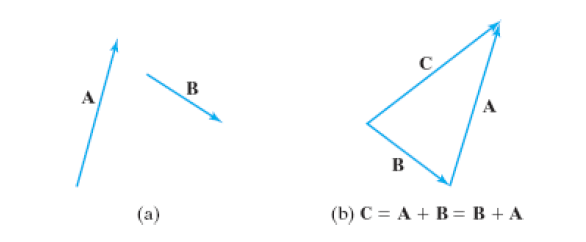
\includegraphics[width=0.7\textwidth]{Figures/5.1.png}
        \caption{两个矢量的和}
        \label{fig:5.1}
    \end{figure}
    \begin{figure}[h!]
        \centering
        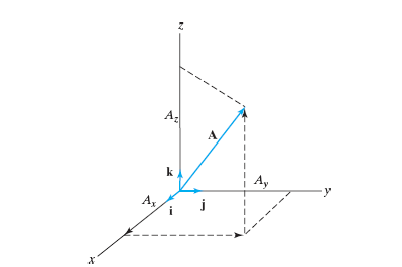
\includegraphics[width=0.7\textwidth]{Figures/5.2.png}
        \caption{单位矢量$\mathrm{i}$、$\mathrm{j}$和$\mathrm{k}$,$\mathrm{A}$的三个分量}
        \label{fig:5.2}
    \end{figure}

    为了获得表示矢量的代数(以及几何)方法,我们在空间中建立了笛卡尔坐标。我们在$x$轴正方向画一个单位矢量,称为$\mathbf{i}$(与虚数单位没有关系)。$y$轴和$z$轴的单位矢量分别称为$\mathbf{j}$和$\mathbf{k}$(图 \ref{fig:5.2})。为了用这三个单位矢量表示空间中的任意矢量$\mathbf{A}$,我们首先将$\mathbf{A}$的起点与原点重合,保持其方向不变。然后,我们找到$\mathbf{A}$在$x$轴、$y$轴和$z$轴上的投影,分别为 $A_x$、$A_y$ 和 $A_z$。由矢量加和的定义,我们有(图 \ref{fig:5.2}):
    \begin{equation}
        \boxed{
            \mathbf{A} = A_x\mathbf{i} + A_y\mathbf{j} + A_z\mathbf{k}
        }
        \label{eq:5.17}
    \end{equation}
    我们可以通过指定$\mathbf{A}$的三个分量($A_x$、$A_y$ 和 $A_z$)来指定矢量 $\mathbf{A}$。因此,三维空间中的矢量可以定义为由三个数组成的有序集合。

    当且仅当两个矢量所有对应的分量都相等时:$A_x = B_x$、$A_y = B_y$ 和 $A_z = B_z$,我们才说这两个向量$\mathbf{A}$和$\mathbf{B}$相等。因此,一个矢量方程等价于三个标量方程。

    为了将两个矢量相加,我们将它们对应的分量相加:
    \begin{equation*}
        \mathbf{A} + \mathbf{B} = A_x\mathbf{i} + A_y\mathbf{j} + A_z\mathbf{k} + B_x\mathbf{i} + B_y\mathbf{j} + B_z\mathbf{k}
    \end{equation*}
    \begin{equation}
        \boxed{
            \mathbf{A} + \mathbf{B} = (A_x + B_x)\mathbf{i} + (A_y + B_y)\mathbf{j} + (A_z + B_z)\mathbf{k}
        }
        \label{eq:5.18}
    \end{equation}
    若$c$是标量,则
    \begin{equation}
        \boxed{
            c\mathbf{A} = cA_x\mathbf{i} + cA_y\mathbf{j} + cA_z\mathbf{k}
        }
        \label{eq:5.19}
    \end{equation}

    矢量$\mathbf{A}$的\textbf{模}(magnitude)为它的长度,由$A$或$\left|\mathbf{A}\right|$表示。模$A$是一个标量。

    两个矢量$\mathbf{A}\cdot\mathbf{B}$的\textbf{点积}(dot product)或\textit{数量积}(scalar product)定义为
    \begin{equation}
        \boxed{
            \mathbf{A}\cdot\mathbf{B} = \left|A\right|\left|B\right|\cos\theta = \mathbf{B}\cdot\mathbf{A}
        }
        \label{eq:5.20}
    \end{equation}
    其中$\theta$是$\mathbf{A}$和$\mathbf{B}$之间的夹角。点积是三个标量的乘积,因此是一个标量。注意$\left|\mathbf{A}\right|\cos\theta$是$\mathbf{A}$在$\mathbf{B}$方向上的投影。根据矢量加法的定义,可以得出矢量 $\mathbf{A}$ + $\mathbf{B}$ 在某个矢量 $\mathbf{C}$ 上的投影是 $\mathbf{A}$ 和 $\mathbf{B}$ 在 $\mathbf{C}$ 上的投影之和。因此,
    \begin{equation}
        \left(\mathbf{A} + \mathbf{B}\right)\cdot\mathbf{C} = \left(\mathbf{A}\cdot\mathbf{C}\right) + \left(\mathbf{B}\cdot\mathbf{C}\right)
        \label{eq:5.21}
    \end{equation}
    由于三个单位矢量 $\mathbf{i}$、$\mathbf{j}$ 和 $\mathbf{k}$ 的长度均为单位长度且互相垂直,我们有
    \begin{equation}
        \mathbf{i}\cdot\mathbf{i} = \mathbf{j}\cdot\mathbf{j} = \mathbf{k}\cdot\mathbf{k} = \cos 0 = 1, \quad \mathbf{i}\cdot\mathbf{j} = \mathbf{i}\cdot\mathbf{k} = \mathbf{j}\cdot\mathbf{k} = \cos \left(\pi/2\right) = 0
        \label{eq:5.22}
    \end{equation}

    使用(\ref{eq:5.22})和分配律(\ref{eq:5.21}),我们有
    \begin{equation*}
        \mathbf{A}\cdot\mathbf{B} = \left(A_x\mathbf{i} + A_y\mathbf{j} + A_z\mathbf{k}\right)\cdot\left(B_x\mathbf{i} + B_y\mathbf{j} + B_z\mathbf{k}\right)
    \end{equation*}
    \begin{equation}
        \boxed{
            \mathbf{A}\cdot\mathbf{B} = A_xB_x + A_yB_y + A_zB_z
        }
        \label{eq:5.23}
    \end{equation}
    其中点积的 9 项中有 6 项为零。

    由式(\ref{eq:5.20})有
    \begin{equation}
        \boxed{
            \mathbf{A}\cdot\mathbf{A} = \left|\mathbf{A}\right|^2
        }
        \label{eq:5.24}
    \end{equation}
    使用式(\ref{eq:5.23}),我们有
    \begin{equation}
        \boxed{
            \left|\mathbf{A}\right| = \left(A_x^2 + A_y^2 + A_z^2\right)^{1/2}
        }
        \label{eq:5.25}
    \end{equation}

    对于三维矢量,还有另一种乘积方式。$\mathbf{A}\times\mathbf{B}$的\textbf{叉积}(cross product)或\textit{向量积}(vector product)是一个新的矢量,其模为
    \begin{equation}
        \mathbf{A}\times\mathbf{B} = \left|\mathbf{A}\right|\left|\mathbf{B}\right|\sin\theta
        \label{eq:5.26}
    \end{equation}
    其线段垂直于$\mathbf{A}$和$\mathbf{B}$所在的平面,其方向与$\mathbf{A}$和$\mathbf{B}$形成一个右手定则的系统(与$x$轴、$y$轴和$z$轴的右手定则相同)。见图 \ref{fig:5.3}。因此,由定义,我们有
    \begin{equation*}
        \mathbf{B}\times\mathbf{A} = -\mathbf{A}\times\mathbf{B}
    \end{equation*}
    同样地(见\textit{Taylor and Mann}, Section 10.2)
    \begin{equation}
        \mathbf{A}\times\left(\mathbf{B}+\mathbf{C}\right) = \mathbf{A}\times\mathbf{B} + \mathbf{A}\times\mathbf{C}
        \label{eq:5.27}
    \end{equation}
    \begin{figure}[h!]
        \centering
        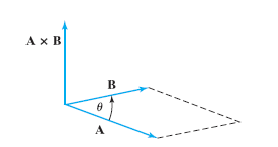
\includegraphics[width=0.4\textwidth]{Figures/5.3.png}
        \caption{两个矢量的叉积}
        \label{fig:5.3}
    \end{figure}
    对于三个单位向量,我们有
    \begin{equation*}
        \mathbf{i}\times\mathbf{i} = \mathbf{j}\times\mathbf{j} = \mathbf{k}\times\mathbf{k} = \sin \: 0 = 0
    \end{equation*}
    \begin{equation*}
        \mathbf{i}\times\mathbf{j} = \mathbf{k}, \quad \mathbf{j}\times\mathbf{i} = -\mathbf{k}, \quad \mathbf{j}\times\mathbf{k} = \mathbf{i}, \quad \mathbf{k}\times\mathbf{j} = -\mathbf{i}, \quad \mathbf{k}\times\mathbf{i} = \mathbf{j}, \quad \mathbf{i}\times\mathbf{k} = -\mathbf{j}
    \end{equation*}
    使用这些等式及分配律(\ref{eq:5.27}),我们有
    \begin{equation*}
        \mathbf{A}\times\mathbf{B} = \left(A_x\mathbf{i} + A_y\mathbf{j} + A_z\mathbf{k}\right)\times\left(B_x\mathbf{i} + B_y\mathbf{j} + B_z\mathbf{k}\right)
    \end{equation*}
    \begin{equation*}
        \mathbf{A}\times\mathbf{B} = \left(A_yB_z - A_zB_y\right)\mathbf{i} + \left(A_zB_x - A_xB_z\right)\mathbf{j} + \left(A_xB_y - A_yB_x\right)\mathbf{k}
    \end{equation*}
    为了便于记忆,我们可以将叉积表示为行列式(见第 8.3 节):
    \begin{equation}
        \mathbf{A}\times\mathbf{B} = \left|
            \begin{array}{ccc}
            \mathbf{i} & \mathbf{j} & \mathbf{k} \\
            A_x & A_y & A_z \\
            B_x & B_y & B_z
            \end{array}
        \right| = \mathbf{i}\left|
            \begin{array}{ccc}
            A_y & A_z \\
            B_y & B_z
            \end{array}
        \right| - \mathbf{j}\left|
            \begin{array}{ccc}
            A_x & A_z \\
            B_x & B_z
            \end{array}
        \right| + \mathbf{k}\left|
            \begin{array}{ccc}
            A_x & A_y \\
            B_x & B_y
            \end{array}
        \right|
        \label{eq:5.28}
    \end{equation}

    我们定义如下的矢量\textbf{微分}(del)算符:
    \begin{equation}
        \boxed{
            \nabla \equiv \mathbf{i}\frac{\partial}{\partial x} + \mathbf{j}\frac{\partial}{\partial y} + \mathbf{k}\frac{\partial}{\partial z}
        }
        \label{eq:5.29}
    \end{equation}
    则由式(\ref{eq:3.23}),线性动量的矢量算符为$\hat{\mathbf{p}}=-\mathrm{i}\hbar\nabla$。

    函数$g\left(x,y,z\right)$的\textbf{梯度}(gradient)定义为将微分算符作用到函数$g$上的结果:
    \begin{equation}
        \boxed{
            \mathbf{grad} \: g\left(x,y,z\right) \equiv \nabla g\left(x,y,z\right) \equiv \mathbf{i}\frac{\partial g}{\partial x} + \mathbf{j}\frac{\partial g}{\partial y} + \mathbf{k}\frac{\partial g}{\partial z}
        }
        \label{eq:5.30}
    \end{equation}
    一个标量函数的梯度为一个矢量函数。矢量$\nabla g\left(x,y,z\right)$代表函数$g$的空间变化率:$\nabla \:g$在$x$方向的分量表示函数$g$在$x$方向的变化率,以此类推。可以证明,矢量$\nabla g$指向 g 变化率最大的方向。由式(\ref{eq:4.24}),势能和力之间的关系为
    \begin{equation}
        \mathbf{F} = -\nabla V\left(x,y,z\right) = -\mathbf{i}\frac{\partial V}{\partial x} - \mathbf{j}\frac{\partial V}{\partial y} - \mathbf{k}\frac{\partial V}{\partial z}
        \label{eq:5.31}
    \end{equation}

    假设某矢量$\mathbf{A}$的三个分量是某参数$t$的函数,即$A_x = A_x\left(t\right)$、$A_y = A_y\left(t\right)$和$A_z = A_z\left(t\right)$。则我们将$\mathbf{A}$对$t$的\textbf{导数}(derivative)定义为
    \begin{equation}
        \frac{\mathrm{d}\mathbf{A}}{\mathrm{d}t} = \mathbf{i}\frac{\mathrm{d}A_x}{\mathrm{d}t} + \mathbf{j}\frac{\mathrm{d}A_y}{\mathrm{d}t} + \mathbf{k}\frac{\mathrm{d}A_z}{\mathrm{d}t}
        \label{eq:5.32}
    \end{equation}

    矢量符号是表示函数变量的一种便捷方法。双粒子系统的波函数可以写作$\psi\left(x_1,y_1,z_1,x_2,y_2,z_2\right)$,如果矢量$\mathbf{r}_1$从原点指向粒子1,那么$\mathbf{r}_1$就具有$x,y,z$三个方向的分量,指定$\mathbf{r}_1$等同于指定三个坐标$x,y,z$。$\mathbf{r}_2$也是如此。因此,我们可以将波函数写成$\psi\left(\mathbf{r}_1,\mathbf{r}_2\right)$。矢量符号也可以用在积分中,例如式(\ref{eq:3.57})对全空间的积分经常写成$\int \cdots \int\left|\Psi\left(\mathbf{r}_1,\cdots,\mathbf{r}_n\right)\right|^2\mathrm{d}\mathbf{r}_1\cdots\mathrm{d}\mathbf{r}_n$。
    
    
\subsection*{$n$维空间的矢量}

    矢量的定义可以推广到三维以上的空间。三维空间中的矢量$\mathbf{A}$可以由其模$\left|\mathbf{A}\right|$和方向来定义;若在笛卡尔坐标系中,还可以用其三个分量$\left(A_x,A_y,A_z\right)$来定义。因此,我们可以把三维矢量定义为按特定顺序排列的三个实数$\left(A_x,A_y,A_z\right)$的集合。$n$ 维实数矢量 “空间”(有时称为超空间)中的矢量 $\mathbf{B}$ 定义为 $n$ 个实数的有序集合$\left(B_1,B_2,\cdots,B_n\right)$,其中$B_1$,$B_2$,$\cdots$,$B_n$是$\mathbf{B}$的\textbf{分量}(components)。不要担心无法将 $n$ 维空间中的矢量可视化。

    函数的变量通常使用 $n$ 维矢量符号表示。例如,在双粒子系统中,与$\psi\left(x_1,y_1,z_1,x_2,y_2,z_2\right)$不同,我们可以定义一个六维矢量$\mathbf{q}$,其分量满足$q_1=x_1, q_2=y_1, q_3=z_1, q_4=x_2, q_5=y_2, q_6=z_2$,且将波函数写成 $\psi\left(\mathbf{q}\right)$。对于有$n$个粒子的系统,我们可以定义一个有$3n$个分量的矢量$\mathbf{q}$,将波函数写成$\psi\left(\mathbf{q}\right)$,使用$\int\left|\psi\left(\mathbf{q}\right)\right|^2\mathrm{d}\mathbf{q}$来进行归一化处理。

    寻找分子平衡几何的理论使用 $n$ 维矢量(第 \ref{sec:15.10 Molecular Geometry} 节)。第 \ref{sec:5.2 Vectors} 节的其余部分与第 \ref{sec:15.10 Molecular Geometry} 节相关,在学习第 \ref{sec:15.10 Molecular Geometry} 节之前不必阅读。

    当且仅当$n$维矢量$\mathbf{B}$和$\mathbf{C}$的所有分量都相等时:$B_1 = C_1$、$B_2 = C_2$、$\cdots$、$B_n = C_n$,我们才说这两个向量\textbf{相等}(equal)。因此,在$n$维空间中,一个矢量方程等价于 $n$ 个标量方程。两个$n$维矢量$\mathbf{B}$与$\mathbf{D}$\textbf{和}(sum)的定义为矢量$\left(B_1+D_1,B_2+D_2,\cdots,B_n+D_n\right)$。矢量的差定义类似。矢量$k\mathbf{B}$定义为矢量$\left(kB_1,kB_2,\cdots,kB_n\right)$,其中 $k$ 是标量。在三维空间中,若$k>0$,则矢量$k\mathbf{A}$的方向一致。在$n$维空间中亦然。与实数对$\left(A_x,A_y,A_z\right)$定义三维空间中的一个点类似,$\left(B_1,B_2,\cdots,B_n\right)$定义$n$维空间中的一个\textbf{点}(point)。

    $n$ 维实数矢量的\textbf{长度}(length)(或\textbf{大小}(magnitude)或\textbf{欧几里得范数}(Euclidean norm))$\left|\mathbf{B}\right|$(有时表示为$\left|\left|\mathbf{B}\right|\right|$ )定义为
    \begin{equation*}
        \left|\mathbf{B}\right| \equiv \left(\mathbf{B}\cdot\mathbf{B}\right)^{1/2} = \left(B_1^2 + B_2^2 + \cdots + B_n^2\right)^{1/2}
    \end{equation*}
    长度为1的矢量称为\textbf{归一化的}(normalized)。

    两个$n$维矢量$\mathbf{B}$和$\mathbf{G}$的\textbf{内积}(inner product)或\textbf{数量积}(scalar product)定义为标量
    \begin{equation*}
        \mathbf{B}\cdot\mathbf{G} \equiv B_1G_1 + B_2G_2 + \cdots + B_nG_n
    \end{equation*}
    若$\mathbf{B}\cdot\mathbf{G}=0$,则称$\mathbf{B}$和$\mathbf{G}$\textbf{正交}(orthogonal)。由式(\ref{eq:5.20}),两个$n$维矢量夹角$\theta$的余弦值定义为$\cos\theta \equiv \left(\mathbf{B}\cdot\mathbf{C}\right)/\left|\mathbf{B}\right|\left|\mathbf{C}\right|$。我们可以证明,这个定义使得 $\theta$ 位于-1 到 1 的范围内。

    在三维空间内,单位矢量$\mathbf{i} = \left(1,0,0\right), \mathbf{j} = \left(0,1,0\right), \mathbf{k} = \left(0,0,1\right)$互相垂直。因此,任意矢量都可以表示为这三个矢量的线性组合[式(\ref{eq:5.17})]。在$n$维空间中,单位矢量$\mathbf{e}_1 \equiv \left(1,0,\cdots,0\right), \mathbf{e}_2 \equiv \left(0,1,\cdots,0\right), \cdots, \mathbf{e}_n \equiv \left(0,0,\cdots,1\right)$互相正交。由于任意$n$维矢量$\mathbf{B}$等于$B_1\mathbf{e}_1 + B_2\mathbf{e}_2 + \cdots + B_n\mathbf{e}_n$,任意$n$维矢量都可以表示为这$n$个单位矢量的线性组合。因此,这 $n$ 个矢量可以说是 $n$ 维实数矢量空间的\textbf{基}(basis)。由于矢量$\mathbf{e_1}, \mathbf{e}_2, \cdots, \mathbf{e}_n$是正交且归一的,它们是这个实矢量空间的\textbf{正交}基(orthonormal basis)。点积$\mathbf{B}\cdot\mathbf{e_i}$给出了矢量 $\mathbf{B}$ 在 $\mathbf{e}_i$ 方向上的分量。矢量空间有许多可能的基集。任何由 $n$ 个线性无关的实矢量组成的集合都可以作为 $n$ 维实矢量空间的基。

    一个三维矢量可以用它的三个分量来指定,也可以用它的长度和方向来指定。可以通过给出矢量与 $x$、$y$ 和 $z$ 轴正半轴所成的三个角度来指定方向。这些角度称为矢量的\textbf{方向角}(direction angles),其值在$0$到$\pi$之间。但是,一旦给出了其他两个方向角,$z$ 轴的方向角就会固定下来,因此只有两个方向角是独立的。因此,一个三维矢量可以用长度和两个方向角来表示。同样,在$n$维空间中,一个矢量和每个单位矢量$\mathbf{e_1},\mathbf{e_2},\cdots,\mathbf{e_n}$之间的方向角也可以根据上述两个矢量之间夹角的余弦公式求出。因此,一个 $n$ 维矢量可以用它的长度和 $n-1$ 个方向角来指定。

    三变量函数的梯度由 (\ref{eq:5.30}) 定义。$n$变量函数$f\left(q_1,q_2,\cdots,q_n\right)$的\textbf{梯度}(gradient)定义为$n$维矢量,其分量分别为$f$对每个变量的一阶偏导数:
    \begin{equation*}
        \nabla f \equiv \left(\partial f/\partial q_1\right)\mathbf{e_1} + \left(\partial f/\partial q_2\right)\mathbf{e}_2 + \cdots + \left(\partial f/\partial q_n\right)\mathbf{e}_n
    \end{equation*}

    我们考虑的是实数 $n$ 维矢量空间。狄拉克(Dirac)对量子力学的表述使用的是复数、无穷维的矢量空间,对它的讨论从略。

\section{单粒子系统的角动量}
\label{sec:5.3 Angular Momentum of a One-Particle System}
    在第\ref{sec:3.3 Operators and Quantum Mechanics}节中,我们找到了线性动量算符$\hat{p}_x$的本征函数和对应的本征值。本节中我们对粒子的角动量进行类似的分析。角动量在原子结构的量子力学中扮演重要的角色。我们从回顾经典力学的角动量开始。

    \subsection*{单粒子的经典力学角动量}
    考虑一个质量为 $m$ 的运动粒子。我们建立一个固定在空间的直角坐标系。设$\mathbf{r}$为从原点指向粒子瞬时位置的矢量,我们有
    \begin{equation}
        \mathbf{r} = \mathbf{i}x + \mathbf{j}y + \mathbf{k}z
        \label{eq:5.33}
    \end{equation}
    其中$x$、$y$ 和 $z$ 是粒子在给定瞬间的坐标。这些坐标是时间的函数。将速度矢量$\mathbf{v}$定义为粒子位置矢量$\mathbf{r}$对时间的导数,我们有[式(\ref{eq:5.32})]
    \begin{equation}
        \mathbf{v} \equiv \frac{\mathrm{d}\mathbf{r}}{\mathrm{d}t} = \mathbf{i}\frac{\mathrm{d}x}{\mathrm{d}t} + \mathbf{j}\frac{\mathrm{d}y}{\mathrm{d}t} + \mathbf{k}\frac{\mathrm{d}z}{\mathrm{d}t}
        \label{eq:5.34}
    \end{equation}
    \begin{equation*}
        v_x = \mathrm{d}x/\mathrm{d}t, \quad v_y = \mathrm{d}y/\mathrm{d}t, \quad v_z = \mathrm{d}z/\mathrm{d}t
    \end{equation*}

    我们定义粒子的\textbf{线性动量}(linear momentum)的矢量$\mathbf{p}$为
    \begin{equation}
        \boxed{
            \mathbf{p} \equiv m\mathbf{v}
        }
        \label{eq:5.35}
    \end{equation}
    \begin{equation}
        p_x = mv_x, \quad p_y = mv_y, \quad p_z = mv_z
        \label{eq:5.36}
    \end{equation}

    粒子相对于坐标原点的\textbf{角动量}(angular momentum)$\mathbf{L}$在经典力学中定义为
    \begin{equation}
        \boxed{
            \mathbf{L} \equiv \mathbf{r} \times \mathbf{p}
        }
        \label{eq:5.37}
    \end{equation}
    \begin{equation}
        \mathbf{L} = \left|
            \begin{array}{ccc}
            \mathbf{i} & \mathbf{j} & \mathbf{k} \\
            x & y & z \\
            p_x & p_y & p_z
            \end{array}
            \right|
        \label{eq:5.38}
    \end{equation}
    \begin{equation}
        L_x = yp_z - zp_y, \quad L_y = zp_x - xp_z, \quad L_z = xp_y - yp_x
        \label{eq:5.39}
    \end{equation}
    其中,我们用到了式(\ref{eq:5.28})。$L_x$、$L_y$ 和 $L_z$ 分别是角动量矢量 $\mathbf{L}$ 在 $x$、$y$ 和 $z$ 方向上的分量。角动量向量的方向垂直于由粒子的位置矢量$\mathbf{r}$和速度矢量$\mathbf{v}$所确定的平面(图\ref{fig:5.4})。
    \begin{figure}[h!]
        \centering
        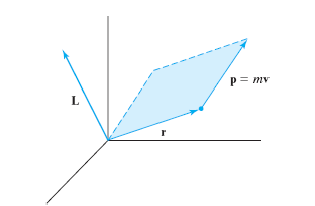
\includegraphics[width=0.5\textwidth]{Figures/5.4.png}
        \caption{$\mathbf{L \equiv \mathbf{r} \times \mathbf{p}}$}
        \label{fig:5.4}
    \end{figure}

    作用在粒子上的\textit{力矩}(torque)$\tau$定义为力$\mathbf{F}$和位置矢量$\mathbf{r}$的叉积:$\tau \equiv \mathbf{r} \times \mathbf{F}$。可以证明:$\tau = \mathrm{d}\mathbf{L} / \mathrm{d}t$。当没有力矩作用于粒子时,其角动量的变化率为零;也就是说,其角动量是恒定的(或守恒的)。对于绕太阳运行的行星来说,引力是沿径向分布的。由于两个平行矢量的交积为零,因此行星上没有力矩,其角动量是守恒的。

\subsection*{单粒子轨道角动量算符}
    现在,让我们来看看量子力学的处理方法。量子力学中有两种角动量。\textbf{轨道角动量}(orbital angular momentum)是粒子在空间运动的结果,与经典力学量 $\mathbf{L}$ 类似。\textbf{自旋角动量}(spin angular momentum)(第\ref{chap:10}章)是许多微观粒子的固有属性,与经典力学没有类似之处。我们现在只考虑轨道角动量。将经典方程(\ref{eq:5.39}) 中的坐标和角动量替换为相应的算符[式 (\ref{eq:3.21})-(\ref{eq:3.23})] ,我们就得到了粒子轨道角动量分量的量子力学算符。有
    \begin{equation}
        \hat{L}_x = -\mathrm{i}\hbar\left(y\frac{\partial}{\partial z} - z\frac{\partial}{\partial y}\right)
        \label{eq:5.40}
    \end{equation}
    \begin{equation}
        \hat{L}_y = -\mathrm{i}\hbar\left(z\frac{\partial}{\partial x} - x\frac{\partial}{\partial z}\right)
        \label{eq:5.41}
    \end{equation}
    \begin{equation}
        \hat{L}_z = -\mathrm{i}\hbar\left(x\frac{\partial}{\partial y} - y\frac{\partial}{\partial x}\right)
        \label{eq:5.42}
    \end{equation}
    (由于$\hat{y}\hat{p}_z = \hat{p}_z\hat{y}$等,我们在构造这些算符时不会遇到不可对易的问题)。使用
    \begin{equation}
        \hat{L}^2 = \left|\hat{\mathbf{L}}\right|^2 = \hat{\mathbf{L}}\cdot\hat{\mathbf{L}} = \hat{L}_x^2 + \hat{L}_y^2 + \hat{L}_z^2
        \label{eq:5.43}
    \end{equation}
    我们可以根据 (\ref{eq:5.40})-(\ref{eq:5.42}) 中的算符构建角动量大小平方的算符。

    由于对易关系决定了哪些物理量可以同时被赋予定值,我们对角动量的对易关系进行了研究。将算符$\hat{L}_y$作用到函数$f\left(x,y,z\right)$上,我们有
    \begin{equation*}
        \hat{L}_yf\left(x,y,z\right) = -\mathrm{i}\hbar\left(z\frac{\partial f}{\partial x} - x\frac{\partial f}{\partial z}\right)
    \end{equation*}
    将$\hat{L}_x$作用到上一个方程上,我们有
    \begin{equation}
        \hat{L}_x\hat{L}_yf = -\hbar^2\left(y\frac{\partial f}{\partial x} + yz \frac{\partial^2f}{\partial z \: \partial x} - yx\frac{\partial^2f}{\partial z^2} - z^2\frac{\partial ^2f}{\partial y \: \partial x} + zx\frac{\partial^2f}{\partial y\: \partial z}\right)
        \label{eq:5.44}
    \end{equation}
    同样地,
    \begin{equation*}
        \hat{L}_xf = -\mathrm{i}\hbar\left(y\frac{\partial f}{\partial z} - z\frac{\partial f}{\partial y}\right)
    \end{equation*}
    将$\hat{L}_y$作用到上一个方程上,我们有
    \begin{equation}
        \hat{L}_y\hat{L}_xf = -\hbar^2\left(zy\frac{\partial^2f}{\partial x\: \partial z}  - z^2\frac{\partial ^2f}{\partial x \: \partial y} - xy\frac{\partial^2f}{\partial z^2} + x\frac{\partial f}{\partial y} + xz \frac{\partial^2f}{\partial z \: \partial y}\right)
        \label{eq:5.45}
    \end{equation}
    (\ref{eq:5.44}) 减去 (\ref{eq:5.45}) ,我们得到
    \begin{equation*}
        \hat{L}_x\hat{L}_yf - \hat{L}_y\hat{L}_xf = -\hbar^2\left(y\frac{\partial f}{\partial x} - x\frac{\partial f}{\partial y}\right)
    \end{equation*}
    \begin{equation}
        \left[\hat{L}_x, \hat{L}_y\right] = \mathrm{i}\hbar\hat{L}_z
        \label{eq:5.46}
    \end{equation}
    其中我们用到了类似以下的关系:
    \begin{equation}
        \boxed{
            \frac{\partial ^2f}{\partial z \: \partial x} = \frac{\partial ^2f}{\partial x \: \partial z}
        }
        \label{eq:5.47}
    \end{equation}
    对于品优函数是正确的。我们可以用相同的过程求出$\left[\hat{L}_y, \hat{L}_z\right]$和$\left[\hat{L}_z, \hat{L}_x\right]$。但我们可以通过注意 (\ref{eq:5.40})-(\ref{eq:5.42}) 中的某种对称性来节省时间。所谓$x$、$y$和$z$的\textbf{循环排列}(cyclic permutation)是指用$y$替换$x$,用$z$替换$y$,用$x$替换$z$。如果我们在$\hat{L}_x$中进行循环排列,就得到了$\hat{L}_y$,在$\hat{L}_y$中进行循环排列就得到了$\hat{L}_z$,在$\hat{L}_z$中进行循环排列就得到了$\hat{L}_x$。因此,对 (\ref{eq:5.46}) 连续进行两次循环置换,就可以得到
    \begin{equation}
        \left[\hat{L}_y, \hat{L}_z\right] = \mathrm{i}\hbar\hat{L}_x, \quad \left[\hat{L}_z, \hat{L}_x\right] = \mathrm{i}\hbar\hat{L}_y
        \label{eq:5.48}
    \end{equation}

    接下来,我们利用第\ref{sec:5.1 Simultaneous Specification of Several Properties}节中对易子的性质,求$\hat{L}^2$和它对应分量的对易子。
    \begin{equation*}
        \begin{aligned}
            \left[\hat{L}^2,\hat{L}_x\right] & = \left[\hat{L}_x^2+\hat{L}_y^2+\hat{L}_z^2,\hat{L}_x\right] \\
            & = \left[\hat{L}_x^2,\hat{L}_x\right] + \left[\hat{L}_y^2,\hat{L}_x\right] + \left[\hat{L}_z^2,\hat{L}_x\right] \\
            & = \left[\hat{L}_y^2,\hat{L}_x\right] + \left[\hat{L}_z^2,\hat{L}_x\right] \\
            & = \hat{L}_y\left[\hat{L}_y,\hat{L}_x\right] + \left[\hat{L}_y,\hat{L}_x\right]\hat{L}_y + \left[\hat{L}_z,\hat{L}_x\right]\hat{L}_z + \hat{L}_z\left[\hat{L}_z,\hat{L}_x\right] \\
            & = -\mathrm{i}\hbar\hat{L}_z\hat{L}_y - \mathrm{i}\hbar\hat{L}_y\hat{L}_z + \mathrm{i}\hbar\hat{L}_y\hat{L}_z + \mathrm{i}\hbar\hat{L}_z\hat{L}_y \\
        \end{aligned} 
    \end{equation*}
    \begin{equation}
        \boxed{
            \left[\hat{L}^2,\hat{L}_x\right] = 0
        }
        \label{eq:5.49}
    \end{equation}
    对$x$、$y$和$z$进行循环替换后,$\hat{L}^2 = \hat{L}_x^2 + \hat{L}_y^2 + \hat{L}_z^2$没有变化,如果对式(\ref{eq:5.49})进行循环替换,我们就可以得到
    \begin{equation}
        \boxed{
            \left[\hat{L}^2,\hat{L}_y\right] = 0, \quad \left[\hat{L}^2,\hat{L}_z\right] = 0
        }
        \label{eq:5.50}
    \end{equation}

    我们可以给$L,L_x,L_y,L_z$中的哪些量赋定值?由于$\hat{L}^2$与其所有分量对应算符均可对易,我们可以为$L^2$和其任意一个分量指定一个精确的值。然而,$\hat{\mathbf{L}}$的任意两个分量之间都不存在对易关系,因此我们不能同时确定多个分量(这个说法有一个例外,稍后讨论)。传统的做法是将 $L_z$ 作为角动量的分量,与 $L^2$ 一起指定。注意:在指定$L^2 = \left|\mathbf{L}\right|^2$的值时,我们并没有指定矢量$\mathbf{L}$的方向。我们只指定了其大小。完整指定$\mathbf{L}$需要同时指定其三个分量,这是我们做不到的。在经典力学中,当角动量守恒时,其三个分量均具有确定的值。而在量子力学中,当角动量守恒时,只有其大小和其中一个分量是确定的。
    \begin{figure}
        \centering
        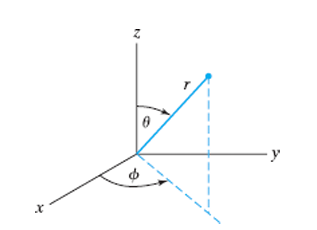
\includegraphics[width=0.4\textwidth]{Figures/5.5.png}
        \caption{球面坐标}
        \label{fig:5.5}
    \end{figure}

    现在,使用这些算符在空间直角坐标系中的形式,我们尝试求出$\hat{L}^2$和$\hat{L}_z$的本征函数和本征值。然而,我们会发现得到的偏微分方程无法分离变量。因此,我们将这些算符转换为\textbf{球面坐标}(spherical coordinate)。坐标$r$表示点$\left(x,y,z\right)$到原点的距离。而角度$\theta$是矢量$\mathbf{r}$与$z$轴正半轴之间的夹角,$\phi$是矢量$\mathbf{r}$在$xOy$平面上的投影与$x$轴正半轴之间的夹角(数学书通常将$\theta$与$\phi$互换)。使用三角法计算,有
    \begin{equation}
        x = r\sin\theta\cos\phi, \quad y = r\sin\theta\sin\phi, \quad z = r\cos\theta
        \label{eq:5.51}
    \end{equation}
    \begin{equation}
        r^2 = x^2 + y^2 + z^2, \quad \cos\theta = \frac{z}{\left(x^2+y^2+z^2\right)^{1/2}}, \quad \tan\phi = \frac{y}{x}
        \label{eq:5.52}
    \end{equation}

    为了将角动量算符转换为球坐标,我们需要对$\partial /\partial x$、$\partial /\partial y$和$\partial /\partial z$进行球坐标变换[如果需要,可以略读这一变换。在 (\ref{eq:5.64}) 之后重新开始阅读]。
    \begin{quote}
        \small 要进行这种变换,我们需要使用\textit{链式法则}(chain rule)。假设我们有一个关于$r$、$\theta$和$\phi$的函数$f\left(r,\theta,\phi\right)$。如果我们改变自变量,将
        \begin{equation*}
            r =r\left(x,y,z\right), \quad \theta = \theta\left(x,y,z\right), \quad \phi = \phi\left(x,y,z\right)
        \end{equation*}
        带入$f$,我们就将其变换为$x$、$y$和$z$的函数
        \begin{equation*}
            f\left[r\left(x,y,z\right),\theta\left(x,y,z\right),\phi\left(x,y,z\right)\right] = g\left(x,y,z\right)
        \end{equation*}
        例如,假设$f\left(r,\theta,\phi\right) = 3r\cos\theta+2\tan^2\phi$。使用式(\ref{eq:5.52}),我们有$g\left(x,y,z\right) = 3z+2y^{2}/x^{2}$。

        链式法则告诉我们$g\left(x,y,z\right)$的偏导数是如何与$f\left(r,\theta,\phi\right)$的偏导数联系起来的。事实上,
        \begin{equation}
            \left(\frac{\partial g}{\partial x}\right)_{y,z} = \left(\frac{\partial f}{\partial r}\right)_{\theta,\phi}\left(\frac{\partial r}{\partial x}\right)_{y,z} + \left(\frac{\partial f}{\partial \theta}\right)_{r,\phi}\left(\frac{\partial \theta}{\partial x}\right)_{y,z} + \left(\frac{\partial f}{\partial \phi}\right)_{r,\theta}\left(\frac{\partial \phi}{\partial x}\right)_{y,z}
            \label{eq:5.53}
        \end{equation}
        \begin{equation}
            \left(\frac{\partial g}{\partial y}\right)_{x,z} = \left(\frac{\partial f}{\partial r}\right)_{\theta,\phi}\left(\frac{\partial r}{\partial y}\right)_{x,z} + \left(\frac{\partial f}{\partial \theta}\right)_{r,\phi}\left(\frac{\partial \theta}{\partial y}\right)_{x,z} + \left(\frac{\partial f}{\partial \phi}\right)_{r,\theta}\left(\frac{\partial \phi}{\partial y}\right)_{x,z}
            \label{eq:5.54}
        \end{equation}
        \begin{equation}
            \left(\frac{\partial g}{\partial z}\right)_{x,y} = \left(\frac{\partial f}{\partial r}\right)_{\theta,\phi}\left(\frac{\partial r}{\partial z}\right)_{x,y} + \left(\frac{\partial f}{\partial \theta}\right)_{r,\phi}\left(\frac{\partial \theta}{\partial z}\right)_{x,y} + \left(\frac{\partial f}{\partial \phi}\right)_{r,\theta}\left(\frac{\partial \phi}{\partial z}\right)_{x,y}
            \label{eq:5.55}
        \end{equation}
        为了将这些方程转换为算符方程,我们删去$f$和$g$,得出
        \begin{equation}
            \frac{\partial}{\partial x} = \left(\frac{\partial r}{\partial x}\right)_{y,z}\frac{\partial}{\partial r} + \left(\frac{\partial \theta}{\partial x}\right)_{y,z}\frac{\partial}{\partial \theta} + \left(\frac{\partial \phi}{\partial x}\right)_{y,z}\frac{\partial}{\partial \phi}
            \label{eq:5.56}
        \end{equation}
        $\partial /\partial y$和$\partial /\partial z$的方程类似。现在的任务是计算类似于$\left(\partial r/\partial x\right)_{y,z}$的偏导数。将(\ref{eq:5.52})中第一个方程在$y$和$z$恒定的条件下对$x$求偏导数,我们有
        \begin{equation*}
            2r\left(\frac{\partial r}{\partial x}\right)_{y,z} = 2x = 2r\sin\theta\cos\phi
        \end{equation*}
        \begin{equation}
            \left(\frac{\partial r}{\partial x}\right)_{y,z} = \sin\theta\cos\phi
            \label{eq:5.57}
        \end{equation}
        将式$r^2 = x^2 + y^2 + z^2$对$y$和$z$求偏导数,我们有
        \begin{equation}
            \left(\frac{\partial r}{\partial y}\right)_{x,z} = \sin\theta\cos\phi, \quad \left(\frac{\partial r}{\partial z}\right)_{x,y} = \cos\theta
            \label{eq:5.58}
        \end{equation}
        由(\ref{eq:5.52})中第二个方程,我们有
        \begin{equation*}
            -\sin\theta\left(\frac{\partial \theta}{\partial x}\right)_{y,z} = -\frac{xz}{r^3}
        \end{equation*}
        \begin{equation}
            \left(\frac{\partial \theta}{\partial x}\right)_{y,z} = \frac{\cos\theta\cos\phi}{r}
            \label{eq:5.59}
        \end{equation}
        同样地,
        \begin{equation}
            \left(\frac{\partial \theta}{\partial y}\right)_{x,z} = \frac{\cos\theta\sin\phi}{r}, \quad \left(\frac{\partial \theta}{\partial z}\right)_{x,y} = -\frac{\sin\theta}{r}
            \label{eq:5.60}
        \end{equation}
        由$\tan\phi = y/x$,我们有
        \begin{equation}
            \left(\frac{\partial\phi}{\partial x}\right)_{y,z} = -\frac{\sin\phi}{r\sin\theta}, \quad \left(\frac{\partial\phi}{\partial y}\right)_{x,z} = \frac{\cos\phi}{r\sin\theta}, \quad \left(\frac{\partial\phi}{\partial z}\right)_{x,y} = 0
            \label{eq:5.61}
        \end{equation}
        将(\ref{eq:5.57})、(\ref{eq:5.59})和(\ref{eq:5.61})代入(\ref{eq:5.56}),我们得到
        \begin{equation}
            \frac{\partial}{\partial x} = \sin\theta\cos\phi\frac{\partial}{\partial r} + \frac{\cos\theta\cos\phi}{r}\frac{\partial}{\partial \theta} - \frac{\sin\phi}{r\sin\theta}\frac{\partial}{\partial \phi}
            \label{eq:5.62}
        \end{equation}
        类似地,我们可以得到
        \begin{equation}
            \frac{\partial}{\partial y} = \sin\theta\sin\phi\frac{\partial}{\partial r} + \frac{\cos\theta\sin\phi}{r}\frac{\partial}{\partial \theta} + \frac{\cos\phi}{r\sin\theta}\frac{\partial}{\partial \phi}
            \label{eq:5.63}
        \end{equation}
        \begin{equation}
            \frac{\partial}{\partial z} = \cos\theta\frac{\partial}{\partial r} - \frac{\sin\theta}{r}\frac{\partial}{\partial \theta}
            \label{eq:5.64}
        \end{equation}
    \end{quote}

    最后,我们可以用球面坐标来表示角动量分量了。将(\ref{eq:5.51})、(\ref{eq:5.63})和(\ref{eq:5.64})带入(\ref{eq:5.40}),得到
    \begin{equation*}
        \begin{aligned}
            \hat{L}_x & = -\mathrm{i}\hbar\left[r\sin\theta\sin\phi\left(\cos\theta\frac{\partial}{\partial r}\right) - \frac{\sin\theta}{r}\frac{\partial }{\partial\theta}\right.\\
            &  \quad \left.-r\cos\theta\left(\sin\theta\sin\phi\frac{\partial}{\partial r} +\frac{\cos\theta\sin\phi}{r}\frac{\partial}{\partial \phi}+\frac{\cos\phi}{r\sin\theta}\frac{\partial}{\partial \phi}\right)\right]
        \end{aligned}
    \end{equation*}
    \begin{equation}
        \hat{L}_x = \mathrm{i}\hbar\left(\sin\phi\frac{\partial}{\partial \theta} - \cos\theta\cos\phi\frac{\partial}{\partial \phi}\right)
        \label{eq:5.65}
    \end{equation}
    同样,我们有
    \begin{equation}
        \hat{L}_y = -\mathrm{i}\hbar\left(\cos\phi\frac{\partial}{\partial \theta} - \cot\theta\sin\phi\frac{\partial}{\partial \phi}\right)
        \label{eq:5.66}
    \end{equation}
    \begin{equation}
        \hat{L}_z = -\mathrm{i}\hbar\frac{\partial}{\partial \phi}
        \label{eq:5.67}
    \end{equation}

    对$\hat{L}_x$、$\hat{L}_y$和$\hat{L}_z$进行平方并相加,我们可以构造出$\hat{L}^2 = \hat{L}_x^2 + \hat{L}_y^2 + \hat{L}_z^2$[式(\ref{eq:5.43})]。结果为(问题5.17)
    \begin{equation}
        \hat{L}^2 = -\hbar^2\left(\frac{\partial^2}{\partial\theta^2} + \cot\theta\frac{\partial}{\partial\theta} + \frac{1}{\sin^2\theta}\frac{\partial^2}{\partial \phi^2}\right)
        \label{eq:5.68}
    \end{equation}

    虽然角动量算符取决于所有三个直角坐标$x$、$y$和$z$,但它们只涉及两个球面坐标$\theta$和$\phi$。

\subsection*{单粒子轨道角动量的本征函数和本征值}
    我们现在希望找到$\hat{L}^2$和$\hat{L}_z$的共同本征函数,记作$Y$。由于这些算符只涉及$\theta$和$\phi$,那么$Y$就是这两个变量的函数:$Y = Y\left(\theta,\phi\right)$(当然,由于这些算符都是线性算符,我们可以用任意一个关于$r$的函数乘以$Y$而不改变$Y$是$\hat{L}^2$和$\hat{L}_z$的本征函数的事实)。我们必须解以下方程:
    \begin{equation}
        \hat{L}_zY\left(\theta,\phi\right) = bY\left(\theta,\phi\right)
        \label{eq:5.69}
    \end{equation}
    \begin{equation}
        \hat{L}^2Y\left(\theta,\phi\right) = cY\left(\theta,\phi\right)
        \label{eq:5.70}
    \end{equation}
    其中$b$和$c$分别是$\hat{L}_z$和$\hat{L}^2$的本征值。

    使用算符$\hat{L}_z$,我们有
    \begin{equation}
        -\mathrm{i}\hbar\frac{\partial}{\partial \phi}Y\left(\theta,\phi\right) = bY\left(\theta,\phi\right)
        \label{eq:5.71}
    \end{equation}
    由于(\ref{eq:5.71})中的算符不涉及$\theta$,我们可以尝试分离变量。将$Y$写成
    \begin{equation}
        Y\left(\theta,\phi\right) = S\left(\theta\right)T\left(\phi\right)
        \label{eq:5.72}
    \end{equation}
    则方程(\ref{eq:5.71})变为
    \begin{equation*}
        -\mathrm{i}\hbar\frac{\partial}{\partial \phi}\left[S\left(\theta\right)T\left(\phi\right)\right] = bS\left(\theta\right)T\left(\phi\right)
    \end{equation*}
    \begin{equation*}
        -\mathrm{i}\hbar S\left(\theta\right)\frac{\mathrm{d}T\left(\phi\right)}{\mathrm{d}\phi} = bS\left(\theta\right)T\left(\phi\right)
    \end{equation*}
    \begin{equation*}
        \frac{\mathrm{d}T\left(\phi\right)}{T\left(\phi\right)} = \frac{\mathrm{i}b}{\hbar}\mathrm{d}\phi
    \end{equation*}
    \begin{equation}
        T\left(\phi\right) = A e^{\mathrm{i}b\phi/\hbar}
        \label{eq:5.73}
    \end{equation}
    其中$A$是任意常数。

    $T$适合作为本征函数吗。答案是否定的,因为它一般不是单值函数。如果我们将$\phi$增加$2\pi$,我们仍将处于空间中的同一点,因此我们希望这样做时 $T$ 保持不变。为了使$T$成为单值函数,我们需要做如下限制:
    \begin{equation*}
        T\left(\phi + 2\pi\right) = T\left(\phi\right)
    \end{equation*}
    \begin{equation*}
        A e^{\mathrm{i}b\phi/\hbar}\mathrm{e}^{\mathrm{i}b2\pi/\hbar} = A e^{\mathrm{i}b\phi/\hbar}
    \end{equation*}
    \begin{equation}
        \mathrm{e}^{\mathrm{i}b2\pi/\hbar} = 1
        \label{eq:5.74}
    \end{equation}

    为了满足$\mathrm{e}^{\mathrm{i}\alpha} = \cos\alpha + \mathrm{i}\sin\alpha = 1$,我们需要$\alpha = 2\pi m$,其中
    \begin{equation*}
        m = 0, \pm 1, \pm 2, \pm\ldots
    \end{equation*}
    因此,由式(\ref{eq:5.74})我们得到
    \begin{equation*}
        2\pi b/\hbar = 2\pi m
    \end{equation*}
    \begin{equation}
        b = m\hbar, \quad m = \ldots, -2, -1, 0, 1, 2, \ldots
        \label{eq:5.75}
    \end{equation}
    式(\ref{eq:5.73})变为
    \begin{equation}
        T\left(\phi\right) = A e^{\mathrm{i}m\phi}, \quad m = 0, \pm 1, \pm 2, \ldots
        \label{eq:5.76}
    \end{equation}
    角动量在$z$方向分量的本征值是量子化的。

    通过归一化$T$,我们可以确定常数$A$。首先,让我们考虑对关于$r$、$\theta$和$\phi$的函数$F$进行归一化。三个独立变量的取值范围是(见图\ref{fig:5.5})
    \begin{equation}
        \boxed{
            0 \le r \le \infty, \quad 0 \le \theta \le \pi, \quad 0 \le \phi < 2\pi
        }
        \label{eq:5.77}
    \end{equation}
    球坐标系下的体积微元为(\textit{Taylor and Mann},第13.9节)
    \begin{equation}
        \boxed{
            \mathrm{d}\tau = r^2\sin\theta \: \mathrm{d}r \: \mathrm{d}\theta \: \mathrm{d}\phi
        }
        \label{eq:5.78}
    \end{equation}
    (\ref{eq:5.78})是一个无限小区域空间的体积,其球面坐标位于$r$到$r+\mathrm{d}r$、$\theta$到$\theta+\mathrm{d}\theta$和$\phi$到$\phi+\mathrm{d}\phi$之间。因此,球坐标下$F$的归一化条件为
    \begin{equation}
        \int_{0}^{\infty}\left[\int_{0}^{\pi}\left[\int_{0}^{2\pi}\left|F\left(r,\theta,\phi\right)\right|^2 \mathrm{d}\phi\right]\sin\theta \mathrm{d}\theta\right]r^2\mathrm{d}r = 1
        \label{eq:5.79}
    \end{equation}
    如果$F$恰好可以写成
    \begin{equation*}
        F\left(r,\theta,\phi\right) = R\left(r\right)S\left(\theta\right)T\left(\phi\right)
    \end{equation*}
    则对(\ref{eq:5.79})使用积分(\ref{eq:3.74}),有
    \begin{equation*}
        \int_{0}^{\infty}\left|R\left(r\right)\right|^2 r^2 \mathrm{d}r \int_{0}^{\pi}\left|S\left(\theta\right)\right|^2 \sin\theta \: \mathrm{d}\theta \int_{0}^{2\pi}\left|T\left(\phi\right)\right|^2 \mathrm{d}\phi = 1
    \end{equation*}
    方便的做法是将$F$的每个因子都作归一化处理:
    \begin{equation}
        \int_{0}^{\infty}\left|R\left(r\right)\right|^2 r^2 \mathrm{d}r = 1, \quad \int_{0}^{\pi}\left|S\left(\theta\right)\right|^2 \sin\theta \: \mathrm{d}\theta = 1, \quad \int_{0}^{2\pi}\left|T\left(\phi\right)\right|^2 \mathrm{d}\phi = 1
        \label{eq:5.80}
    \end{equation}
    因此,
    \begin{equation*}
        \int_{0}^{2\pi}\left(A\mathrm{e}^{\mathrm{i}m\phi}\right)^{\ast}\left(A\mathrm{e}^{\mathrm{i}m\phi}\right) \mathrm{d}\phi = 1 = \left|A\right|^2\int_{0}^{2\pi} \mathrm{d}\phi
    \end{equation*}
    \begin{equation*}
        \left|A\right| = \left(2\pi\right)^{-1/2}
    \end{equation*}
    \begin{equation}
        T\left(\phi\right) = \frac{1}{\sqrt{2\pi}}e^{\mathrm{i}m\phi}, \quad m = 0, \pm 1, \pm 2, \ldots
        \label{eq:5.81}
    \end{equation}

    我们现在尝试使用式(\ref{eq:5.70})来求解$\hat{L}^2$的本征值$c$。对$\hat{L}^2$使用式(\ref{eq:5.68})、对$Y$使用式(\ref{eq:5.72}),由式(\ref{eq:5.81}),我们有
    \begin{equation*}
        -\hbar^2\left(\frac{\partial^2}{\partial\theta^2} + \cot\theta\frac{\partial}{\partial\theta} + \frac{1}{\sin^2\theta}\frac{\partial^2}{\partial\phi^2}\right)\left(S\left(\theta\right)\frac{1}{\sqrt{2\pi}}e^{\mathrm{i}m\phi}\right) = cS\left(\theta\right)\frac{1}{\sqrt{2\pi}}e^{\mathrm{i}m\phi}
    \end{equation*}
    \begin{equation}
        \frac{\mathrm{d}^2S}{\mathrm{d}\theta^2}+\cot\theta\frac{\mathrm{d}S}{\mathrm{d}\theta} - \frac{m^2}{\sin^2\theta}S = -\frac{c}{\hbar^2}S
        \label{eq:5.82}
    \end{equation}
    \begin{quote}
        \small
        \noindent 为了解方程(\ref{eq:5.82}),我们需要进行一些繁琐的操作,如果需要,可以略过不读。在式(\ref{eq:5.91})处重新开始阅读。首先,为了方便起见,我们将自变量代替为
        \begin{equation}
            w = \cos\theta
            \label{eq:5.83}
        \end{equation}
        将$S$变换为一个新的关于$w$的函数:
        \begin{equation}
            S\left(\theta\right) = G\left(w\right)
            \label{eq:5.84}
        \end{equation}
        由链式法则,我们有
        \begin{equation}
            \frac{\mathrm{d}S}{\mathrm{d}\theta} = \frac{\mathrm{d}G}{\mathrm{d}w}\frac{\mathrm{d}w}{\mathrm{d}\theta} = -\sin\theta\frac{\mathrm{d}G}{\mathrm{d}w} = -\left(1-w^2\right)^{1/2}\frac{\mathrm{d}G}{\mathrm{d}w}
            \label{eq:5.85}
        \end{equation}
        同样地,我们得出(问题5.25)
        \begin{equation}
            \frac{\mathrm{d}^2S}{\mathrm{d}\theta^2} = \left(1-w^2\right)\frac{\mathrm{d}^2G}{\mathrm{d}w^2} - w\frac{\mathrm{d}G}{\mathrm{d}w}
            \label{eq:5.86}
        \end{equation}
        由式(\ref{eq:5.86})、(\ref{eq:5.85})和$\cot\theta = \cos\theta/\sin\theta = w/\left(1-w^2\right)^{1/2}$,我们可以将(\ref{eq:5.82})重写为
        \begin{equation}
            \left(1-w^2\right)\frac{\mathrm{d}^2G}{\mathrm{d}w^2} - 2w\frac{\mathrm{d}G}{\mathrm{d}w}+\left[\frac{c}{\hbar^2}-\frac{m^2}{1-w^2}\right]G\left(w\right) = 0
            \label{eq:5.87}
        \end{equation}
        $w$的取值范围是$-1 \le w \le 1$。

        在尝试幂级数求解时,为了得到两项的递推关系,我们需要对因变量作如下改变:
        \begin{equation}
            G\left(w\right) = \left(1-w^2\right)^{\left|m\right|/2}H\left(w\right)
            \label{eq:5.88}
        \end{equation}
        对(\ref{eq:5.88})求导,我们得到了$G^{\prime}$和$G^{\prime\prime}$,在除以$\left(1-w^2\right)^{\left|m\right|/2}$后,我们可以将(\ref{eq:5.87})变为
        \begin{equation}
            \left(1-w^2\right)H^{\prime\prime} - 2\left(\left|m\right|+1\right)wH^{\prime} + \left[c\hbar^{-2}-\left|m\right|\left(\left|m\right|+1\right)\right]H = 0
            \label{eq:5.89}
        \end{equation}
        现在,我们尝试$H$的幂级数解
        \begin{equation}
            H\left(w\right) = \sum_{n=0}^{\infty}a_jw^j
            \label{eq:5.90}
        \end{equation}
        对其求导[与式(\ref{eq:4.36})-(\ref{eq:4.38})类似],我们有
        \begin{equation*}
            H^{\prime}\left(w\right) = \sum_{j=0}^{\infty}ja_jw^{j-1}
        \end{equation*}
        \begin{equation*}
            H^{\prime\prime}\left(w\right) = \sum_{j=0}^{\infty}j(j-1)a_jw^{j-2} = \sum_{j=0}^{\infty}\left(j+2\right)\left(j+1\right)a_{j+2}w^{j}
        \end{equation*}
        将这些幂级数带入式(\ref{eq:5.89}),合并求和后,有
        \begin{equation*}
            \sum_{j=0}^{\infty}\left[\left(j+2\right)\left(j+1\right)a_{j+2}+\left(-j^2-j-2\left|m\right|j+\frac{c}{\hbar^2}-\left|m\right|^2-\left|m\right|\right)a_j\right]w^j=0
        \end{equation*}
        令$w^j$的系数为零,我们得到
        \begin{equation}
            a_{j+2} = \frac{\left(j+\left|m\right|\right)\left(j+\left|m\right|+1\right)-c/\hbar^{-2}}{\left(j+1\right)\left(j+2\right)}a_j
            \label{eq:5.91}
        \end{equation}
    \end{quote}

    与谐振子的例子一样,式(\ref{eq:5.89})的通解也是偶次幂级数(系数由$a_0$决定)和奇次幂级数(系数由$a_1$决定)的任意线性组合。可以证明,由式(\ref{eq:5.91})定义的无穷级数不是品优函数。[许多文献都指出:该级数在$w = \pm 1$处发散。然而,这并不足以否定该无穷级数,因为本征函数是平方可积的,即使在某两点上是无穷的。仔细讨论见 M. Whippman, Am. Phys., 34, 656 (1966)。]因此,与谐振子的情况一致,我们必须让级数在某一项$a_kw^k$处打断。根据$k$是奇数还是偶数,我们设$a_0$或$a_1$为零,从而消除其他级数。

    令式(\ref{eq:5.91})中$a_k$的系数为零,得到
    \begin{equation}
        c = \hbar^2\left(k+\left|m\right|\right)\left(k+\left|m\right|+1\right), \quad k = 0, 1, 2, \ldots
        \label{eq:5.92}
    \end{equation}
    由于$\left|m\right|$的值为$0, 1, 2, \ldots$,$k+\left|m\right|$的值为$0, 1, 2, \ldots$。因此,我们可以定义量子数$l$为
    \begin{equation}
        l = k + \left|m\right|
        \label{eq:5.93}
    \end{equation}
    角动量大小平方的本征值为
    \begin{equation}
        c = l\left(l+1\right)\hbar^2, \quad l = 0, 1, 2, \ldots
        \label{eq:5.94}
    \end{equation}
    单粒子轨道角动量的大小为
    \begin{equation}
        \left|\mathbf{L}\right| = \left[l\left(l+1\right)\right]^{1/2}\hbar
        \label{eq:5.95}
    \end{equation}

    由式(\ref{eq:5.93})有$\left|m\right| = l$。因此,$m$的取值范围为
    \begin{equation}
        m = -l, -l+1, -l+2, \ldots, -1, 0, 1, \ldots, l-2, l-1, l, l
        \label{eq:5.96}
    \end{equation}

    现在让我们检查角动量的本征函数。由式(\ref{eq:5.83})、(\ref{eq:5.84})、(\ref{eq:5.88})、(\ref{eq:5.90})和(\ref{eq:5.93}),本征函数中的$\theta$因子为
    \begin{equation}
        S_{l,m}\left(\theta\right) = \sin^{\left|m\right|}\theta\sum_{\substack{j=1,3,\ldots \\ j=0,2,\ldots}}^{l-\left|m\right|}a_j\cos^j\theta
        \label{eq:5.97}
    \end{equation}
    其中,$l-\left|m\right|$的奇偶性决定求和从$j=1$还是$j=0$开始。使用式(\ref{eq:5.94}),$a_j$的系数满足的递推关系(\ref{eq:5.91})可以写成
    \begin{equation}
        a_{j+2} = \frac{\left(j+\left|m\right|\right)\left(j+\left|m\right|+1\right)-l\left(l+1\right)}{\left(j+1\right)\left(j+2\right)}a_j
        \label{eq:5.98}
    \end{equation}

    $\hat{L}^2$和$\hat{L}_z$的本征函数由式(\ref{eq:5.72})和式(\ref{eq:5.81})给出:
    \begin{equation}
        \boxed{
            Y^m_l\left(\theta,\phi\right) = S_{l,m}\left(\theta\right)T\left(\phi\right) = \frac{1}{\sqrt{2\pi}}S_{l,m}\left(\theta\right)e^{\mathrm{i}m\phi}
        }
        \label{eq:5.99}
    \end{equation}
    $Y^m_l$中的$m$是一个标签,而不是指数。
    \begin{examplebox}
        \textbf{例题:}分别求当(a)$l=0$;(b)$l=1$时$Y_l^m\left(\theta,\phi\right)$、$\hat{L}^2$和$\hat{L}_z$的本征值。
        \\

        \textbf{(a)}对于$l=0$,由式(\ref{eq:5.96}),有$m=0$。则式(\ref{eq:5.97})变为
        \begin{equation}
            S_{0,0}\left(\theta\right) = a_0
            \label{eq:5.100}
        \end{equation}
        由归一化条件(\ref{eq:5.80}),我们有
        \begin{equation*}
            \int_{0}^{\pi}\left|a_0\right|^2 \sin\theta \: \mathrm{d}\theta = 1 = 2\left|a_0\right|^2
        \end{equation*}
        \begin{equation*}
            \left|a_0\right| = 2^{-1/2}
        \end{equation*}
        则式(\ref{eq:5.99})变为
        \begin{equation}
            Y^0_0\left(\theta,\phi\right) = \frac{1}{\sqrt{4\pi}}
            \label{eq:5.101}
        \end{equation}
        [显然,式(\ref{eq:5.101})是$\hat{L}^2$、$\hat{L}_x$、$\hat{L}_y$和$\hat{L}_z$的本征函数,方程(\ref{eq:5.65})-(\ref{eq:5.68})。]对于$l=0$,本征函数不存在角度依赖关系,我们说本征函数是\textbf{球对称的}(spherically symmetric)。

        对于$l=0$和$m=0$,由式(\ref{eq:5.69})、(\ref{eq:5.70})、(\ref{eq:5.75})和(\ref{eq:5.94}),我们有$\hat{L}^2$的本征值为$c=0$,$\hat{L}_z$的本征值为$b=0$。

        \textbf{(b)} 对于$l=1$,由式(\ref{eq:5.96}),有$m=-1, 0, 1$。当$\left|m\right| = 1$时,式(\ref{eq:5.97})变为
        \begin{equation}
            S_{1,\pm 1}\left(\theta\right) = a_0\sin\theta
            \label{eq:5.102}
        \end{equation}
        (\ref{eq:5.102})中的$a_0$和(\ref{eq:5.100})中的$a_0$不一定相等。由归一化条件,有
        \begin{equation*}
            1 = \left|a_0^2\right|\int_{0}^{\pi}\sin^2\theta\sin\theta \: \mathrm{d}\theta = \left|a_0^2\right|\int_{-1}^{1}\left(1-w^2\right) \: \mathrm{d}w
        \end{equation*}
        \begin{equation*}
            \left|a_0\right| = \sqrt{3}/2
        \end{equation*}
        其中,我们将$w$用$\cos\theta$代替。因此,我们有$S_{1,\pm 1}\left(3^{1/2}/2\right)\sin\theta$,式(\ref{eq:5.99})变为
        \begin{equation}
            Y_1^1 = \left(3/8\pi\right)^{1/2}\sin\theta e^{\mathrm{i}\phi}, \quad Y_1^{-1} = \left(3/8\pi\right)^{1/2}\sin\theta e^{-\mathrm{i}\phi}
            \label{eq:5.103}
        \end{equation}
        当$l=1$而$m=0$时,我们得出(见下文的练习题)$S_{1,0} = \left(3/2\right)^{1/2}\cos\theta$,$Y_1^0 = \left(3/4\pi\right)^{1/2}\cos\theta$。因此,当$l=1$时,由式(\ref{eq:5.94})可得$\hat{L}^2$的本征值为$2\hbar^2$;由式(\ref{eq:5.75}),$\hat{L}_z$的本征值为$\hbar$、$0$和$-\hbar$,分别与$m=1, 0, -1$对应。
        \\

        \textbf{练习:}验证$S_{1,0}$和$Y_1^0$的表达式。
    \end{examplebox}

    函数$S_{l,m}\left(\theta\right)$在数学中是众所周知的,是乘以一个归一化系数后的\textit{连带勒让德函数}(associated Legendre function)。连带勒让德函数的定义见问题5.34。表(\ref{tab:5.1})列出了$l \le 3$的$S_{l,m}\left(\theta\right)$表达式。
    \begin{table}[htbp]
        \centering
        \caption{$S_{l,m}\left(\theta\right)$}
        \label{tab:5.1}
        \begin{tabular}{|l|l|}
            \hline
            $l=0$: & $S_{0,0} = \frac{1}{2}\sqrt{2}$ \\
            \hline
            $l=1$: & $S_{1,0} = \frac{1}{2}\sqrt{6}\cos\theta$ \\
            & $S_{1,\pm 1} = \frac{1}{2}\sqrt{3}\sin\theta$ \\
            \hline
            $l=2$: & $S_{2,0} = \frac{1}{4}\sqrt{10}\left(3\cos^2\theta - 1\right)$ \\
            & $S_{2,\pm 1} = \frac{1}{2}\sqrt{15}\sin\theta\cos\theta$ \\
            & $S_{2,\pm 2} = \frac{1}{4}\sqrt{15}\sin^2\theta$ \\
            \hline
            $l=3$: & $S_{3,0} = \frac{3}{4}\sqrt{14}\left(\frac{5}{3}\cos^3\theta-\cos\theta\right)$ \\
            & $S_{3, \pm 1} = \frac{1}{8}\sqrt{42}\sin\theta\left(5\cos^2\theta - 1\right)$ \\
            & $S_{3, \pm 2} = \frac{1}{4}\sqrt{105}\sin^2\theta\cos\theta$ \\
            & $S_{3, \pm 3} = \frac{1}{8}\sqrt{70}\sin^3\theta$ \\
            \hline
        \end{tabular}
    \end{table}
    \begin{equation}
        \boxed{
            \hat{L}^2Y^m_l\left(\theta,\phi\right) = l\left(l+1\right)\hbar^2Y^m_l\left(\theta,\phi\right), \quad l = 0, 1, 2, \ldots
        }
        \label{eq:5.104}
    \end{equation}
    \begin{equation}
        \boxed{
            \hat{L}_zY^m_l\left(\theta,\phi\right) = m\hbar Y^m_l\left(\theta,\phi\right), \quad m = -l, -l+1, \ldots, l-1, l
        }
        \label{eq:5.105}
    \end{equation}
    其中,本征函数由式(\ref{eq:5.99})给出。我们通常使用符号$m_l$代替$m$来表示$L_z$量子数。我们稍后会看到球谐函数是正交函数(方程7.27)。

    由于$l \ge \left|m\right|$,因此除了$l=0$以外,轨道角动量$\mathbf{L}$的大小$\left[l\left(l+1\right)\right]^{1/2}\hbar^2$大于其$z$方向的分量$\left|m\right|\hbar$。如果可以让角动量的大小等于其 $z$ 分量,这就意味着 $x$ 和 $y$ 分量为零,我们就可以指定 $\mathbf{L}$ 的所有三个分量了。然而这是做不到的,因为角动量三个分量的算符不可对易。只有一种例外,就是$l$为零时。在该情况中,$\left|\mathbf{L}\right|^2 = L_x^2+ L_y^2 + L_z^2 = 0$,因此所有三个分量都为零。由式(\ref{eq:5.12}),角动量分量的不确定性满足
    \begin{equation}
        \Delta L_x\Delta L_y \ge \left|\frac{1}{2}\Psi^{\ast}\left[\hat{L}_x,\hat{L}_y\right]\Psi\mathrm{d}\tau\right| = \frac{\hbar}{2}\left|\int \Psi^{\ast}\hat{L}_z\Psi\mathrm{d}\tau\right|
        \label{eq:5.106}
    \end{equation}
    通过循环排列能得出其余两个相似的方程。当$\hat{L}_x$、$\hat{L}_y$和$\hat{L}_z$的本征值为零时,$\hat{L}_x\Psi = 0$,$\hat{L}_y\Psi = 0$,$\hat{L}_z\Psi = 0$,式(\ref{eq:5.106})的右侧和另两个相似的方程也为零,因此$\Delta L_x = \Delta L_y = \Delta L_z = 0$被允许。然而,根据第\ref{sec:5.1 Simultaneous Specification of Several Properties}节,要同时得到两个算符的本征函数,这两个算符必须可对易,这又是怎么回事呢?答案是,这个定理指的是一个算符的整套本征函数是另一个算符的本征函数的可能性。因此,尽管$\hat{L}_x$和$\hat{L}_z$不可对易,但仍有可能使得$\hat{L}_x$的本征函数同时也是$\hat{L}_z$的本征函数($l=0=m$时)。然而,使得$\hat{L}_x$的\textit{所有}本征函数都是$\hat{L}_z$的本征函数是不可能的。
    \begin{figure}[h!]
        \centering
        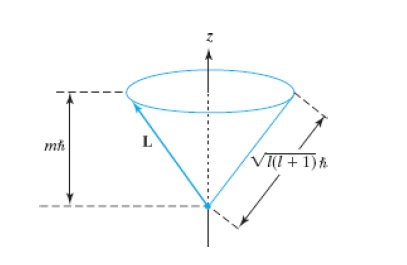
\includegraphics[width=0.5\textwidth]{Figures/5.6.png}
        \caption{$\mathbf{L}$的方向}
        \label{fig:5.6}
    \end{figure}
    \begin{figure}
        \centering
        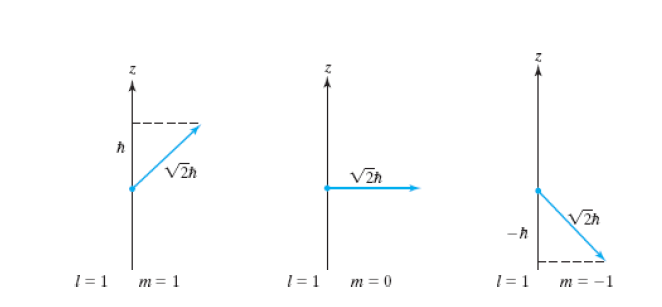
\includegraphics[width=0.5\textwidth]{Figures/5.7.png}
        \caption{$l=1$时$\mathbf{L}$相对于$z$轴的方向}
        \label{fig:5.7}
    \end{figure}

    由于我们无法指定$L_x$和$L_y$,所以矢量$\mathbf{L}$可以位于以$z$轴为轴,高度为$m\hbar$的圆锥面上的任何位置。当$l=1$时,$\mathbf{L}$相对于$z$轴的可能方向如图\ref{fig:5.7}所示。对于每一个$\hat{L}^2$的本征值,都有$2l+1$个不同的本征函数$Y_l^m$,与$m$的$2l+1$个取值相对应。我们说$\hat{L}^2$的本征值是$\left(2l+1\right)$重简并的,\textbf{简并}(degeneracy)一词适用于任何算符的本征值,而不仅仅是哈密顿算符。

    当然,$z$轴并没有什么特别之处。空间中的所有方向都是等价的。如果我们选择确定$L^2$和$L_x$(而不是$L_z$),我们会得到与$L_z$相同的$L_x$的本征值。然而,解$\hat{L}_z$的本征方程更为简单,因为在球坐标系中,$\hat{L}_z$的形式更简单,其中涉及到围绕$z$轴的旋转角度$\phi$。

\section{角动量阶梯算符法}
\label{sec:5.4 The Ladder-Operator Method for Angular Momentum}
    通过将轨道角动量的算符表示为微分算符,并求解由此产生的微分方程,我们得到了$\hat{L}^2$和$\hat{L}_z$的本征值。我们现在证明:只需要利用算符之间的对易关系就能找到这些本征值。本节的工作适用于任何满足角动量对易关系的算符。它尤其适用于自旋角动量(第 \ref{chap:10} 章)和轨道角动量。

    我们使用字母$L$来表示轨道角动量。在这里,我们将使用字母 $M$ 来表示我们正在处理的任何一种角动量。我们有三个线性算符$\hat{M}_x$、$\hat{M}_y$和$\hat{M}_z$,我们只知道它们符合对易关系[与式(\ref{eq:5.46})和(\ref{eq:5.48})相似]
    \begin{equation}
        \left[\hat{M}_x,\hat{M}_y\right] = \mathrm{i}\hbar\hat{M}_z, \quad \left[\hat{M}_y,\hat{M}_z\right] = \mathrm{i}\hbar\hat{M}_x, \quad \left[\hat{M}_z,\hat{M}_x\right] = \mathrm{i}\hbar\hat{M}_y
        \label{eq:5.107}
    \end{equation}
    我们定义算符$\hat{M}^2$为
    \begin{equation}
        \hat{M}^2 = \hat{M}_x^2 + \hat{M}_y^2 + \hat{M}_z^2
        \label{eq:5.108}
    \end{equation}
    我们的问题是如何找到$\hat{M}^2$和$\hat{M}_z$的本征值。

    使用式(\ref{eq:5.107})和(\ref{eq:5.108}),我们从对$\hat{M}^2$及其分量的对易子进行评估开始。与推导(\ref{eq:5.49})和(\ref{eq:5.50})时的推导类似,我们有
    \begin{equation}
        \left[\hat{M}^2,\hat{M}_x\right] = \left[\hat{M}^2,\hat{M}_y\right] = \left[\hat{M}^2,\hat{M}_z\right] = 0
        \label{eq:5.109}
    \end{equation}
    因此,我们可以得到$\hat{M}^2$和$\hat{M}_z$的同时本征函数。

    现在我们定义两个新算符,\textbf{升算符}(raising operator)$\hat{M}_+$和\textbf{降算符}(lowering operator)$\hat{M}_-$,它们的定义为
    \begin{equation}
        \hat{M}_+ \equiv \hat{M}_x + \mathrm{i}\hat{M}_y
        \label{eq:5.110}
    \end{equation}
    \begin{equation}
        \hat{M}_- \equiv \hat{M}_x - \mathrm{i}\hat{M}_y
        \label{eq:5.111}
    \end{equation}
    这些是\textbf{阶梯算符}(ladder operator)的例子。使用这些术语的原因很快就会清楚。我们有
    \begin{equation*}
        \begin{aligned}
            \hat{M}_+\hat{M}_- & = \left(\hat{M}_x+\mathrm{i}\hat{M}_y\right)\left(\hat{M}_x-\mathrm{i}\hat{M}_y\right) = \hat{M}_x\left(\hat{M}_x-\mathrm{i}\hat{M}_y\right) + \mathrm{i}\hat{M}_y\left(\hat{M}_x-\mathrm{i}\hat{M}_y\right) \\
            & = \hat{M}_x^2 - \mathrm{i}\hat{M}_x\hat{M}_y + \mathrm{i}\hat{M}_y\hat{M}_x + \hat{M}_y^2 = \hat{M}^2 - \hat{M}_z^2 + \mathrm{i}\left[\hat{M}_y,\hat{M}_x\right]
        \end{aligned}
    \end{equation*}
    \begin{equation}
        \hat{M}_+\hat{M}_- = \hat{M}^2 - \hat{M}_z^2 + \hbar\hat{M}_z
        \label{eq:5.112}
    \end{equation}
    同样地,我们有
    \begin{equation}
        \hat{M}_-\hat{M}_+ = \hat{M}^2 - \hat{M}_z^2 - \hbar\hat{M}_z
        \label{eq:5.113}
    \end{equation}
    对于这些算符与$\hat{M}_z$的对易子,我们有
    \begin{equation*}
        \left[\hat{M}_+,\hat{M}_z\right] = \left[\hat{M}_x+\mathrm{i}\hat{M}_y,\hat{M}_z\right] = \left[\hat{M}_x,\hat{M}_z\right]+\mathrm{i}\left[\hat{M}_y,\hat{M}_z\right] = -\mathrm{i}\hbar\hat{M}_y - \hbar\hat{M}_x
    \end{equation*}
    \begin{equation*}
        \left[\hat{M}_+,\hat{M}_z\right] = -\hbar\hat{M}_+
    \end{equation*}
    \begin{equation}
        \hat{M}_+\hat{M}_z = \hat{M}_z\hat{M}_+ - \hbar\hat{M}_+
        \label{eq:5.114}
    \end{equation}
    其中我们用到了式(\ref{eq:5.107})。同样地,我们有
    \begin{equation}
        \hat{M}_-\hat{M}_z = \hat{M}_z\hat{M}_- + \hbar\hat{M}_-
        \label{eq:5.115}
    \end{equation}

    设$Y$是$\hat{M}^2$和$\hat{M}_z$的共同本征函数,即
    \begin{equation}
        \hat{M}^2Y = cY
        \label{eq:5.116}
    \end{equation}
    \begin{equation}
        \hat{M}_zY = bY
        \label{eq:5.117}
    \end{equation}
    其中$c$和$b$是本征值。将算符$\hat{M}_+$作用于式(\ref{eq:5.117}),我们有
    \begin{equation*}
        \hat{M}_+\hat{M}_zY = \hat{M}_+bY
    \end{equation*}
    使用式(\ref{eq:5.114}),及$\hat{M}_+$是线性算符,我们有
    \begin{equation*}
        \left(\hat{M}_z\hat{M}_+-\hbar\hat{M}_+\right)Y = b\hat{M}_+Y
    \end{equation*}
    \begin{equation}
        \hat{M}_z\left(\hat{M}_+Y\right) = \left(b+\hbar\right)\left(\hat{M}_+Y\right)
        \label{eq:5.118}
    \end{equation}
    最后一个方程说明:$\hat{M}_+Y$是算符$\hat{M}_z$的本征函数,其本征值为$b+\hbar$。换句话说,将升算符$\hat{M}_+$作用到本征函数$Y$上后,可以将$Y$转换成另一个$\hat{M}_z$的本征函数,其本征值比$Y$的大$\hbar$。如果我们现在对式(\ref{eq:5.118})使用升算符,并再次使用式(\ref{eq:5.114}),我们得到
    \begin{equation*}
        \hat{M}_z\left(\hat{M}_+^2Y\right) = \left(b+2\hbar\right)\left(\hat{M}_+^2Y\right)
    \end{equation*}
    重复应用升算符,有
    \begin{equation}
        \hat{M}_z\left(\hat{M}_+^kY\right) = \left(b+k\hbar\right)\left(\hat{M}_+^kY\right), \quad k = 0, 1, 2, \ldots
        \label{eq:5.119}
    \end{equation}

    如果我们对式(\ref{eq:5.117})使用降算符$\hat{M}_-$并应用式(\ref{eq:5.115}),我们已同样的方式发现:
    \begin{equation}
        \hat{M}_z\left(\hat{M}_-Y\right) = \left(b-\hbar\right)\left(\hat{M}_-Y\right)
        \label{eq:5.120}
    \end{equation}
    \begin{equation}
        \hat{M}_z\left(\hat{M}_-^kY\right) = \left(b-k\hbar\right)\left(\hat{M}_-^kY\right)
        \label{eq:5.121}
    \end{equation}

    这样,通过对本征值为$b$的本征函数使用升降算符,我们得到了一个本征值阶梯,阶梯之间的差值为$\hbar$:
    \begin{equation*}
        \ldots, \quad b-2\hbar, \quad b-\hbar, \quad b, \quad b+\hbar, \quad b+2\hbar, \quad \ldots
    \end{equation*}
    函数$\hat{M}_{\pm}^kY$是$\hat{M}_z$的本征函数,其本征值为$b \pm k\hbar$[式(\ref{eq:5.119})和(\ref{eq:5.121})]。我们现在表明这些函数也是$\hat{M}^2$的本征函数,其本征值为$c$:
    \begin{equation}
        \hat{M}_z\hat{M}_{\pm}^kY = \left(b \pm k\hbar\right)\hat{M}_{\pm}^kY
        \label{eq:5.122}
    \end{equation}
    \begin{equation}
        \hat{M}^2\hat{M}_{\pm}^kY = c\hat{M}_{\pm}^kY
        \label{eq:5.123}
    \end{equation}
    为了证明(\ref{eq:5.123}),我们首先表明$\hat{M}^2$与$\hat{M}_+$和$\hat{M}_-$对易。我们有
    \begin{equation*}
        \left[\hat{M}^2,\hat{M}_{\pm}\right] = \left[\hat{M}^2,\hat{M}_x\pm\mathrm{i}\hat{M}_y\right] = \left[\hat{M}^2,\hat{M}_x\right] \pm \mathrm{i}\left[\hat{M}^2,\hat{M}_y\right] = 0 \pm 0 = 0
    \end{equation*}
    也有
    \begin{equation*}
        \left[\hat{M}^2,\hat{M}_{\pm}^2\right] = \left[\hat{M}^2,\hat{M}_{\pm}\right]\hat{M}_{\pm} + \hat{M}_{\pm}\left[\hat{M}^2,\hat{M}_{\pm}\right] = 0 + 0 = 0
    \end{equation*}
    通过归纳法可以得出
    \begin{equation}
        \left[\hat{M}^2,\hat{M}_{\pm}^k\right] = 0, \quad \text{或} \quad \hat{M}^2\hat{M}_{\pm}^k = \hat{M}_{\pm}^k\hat{M}^2, \quad k = 0, 1, 2, \ldots
        \label{eq:5.124}
    \end{equation}
    如果我们对式(\ref{eq:5.116})使用升降算符$\hat{M}_{\pm}$,并使用(\ref{eq:5.124}),我们有
    \begin{equation*}
        \hat{M}_{\pm}^k\hat{M}^2Y = \hat{M}_{\pm}^k cY
    \end{equation*}
    \begin{equation}
        \hat{M}^2\left(\hat{M}_{\pm}^kY\right) = c\left(\hat{M}_{\pm}^kY\right)
        \label{eq:5.125}
    \end{equation}
    这正是我们想要证明的。

    接下来我们想证明:使用阶梯算符生成的$\hat{M}_z$的本征值集合是有界的。对于特定的,本征值为$b$的算符$\hat{M}_z$的本征函数$Y$,我们有
    \begin{equation*}
        \hat{M}_zY = bY
    \end{equation*}
    若考虑由阶梯算符生成的本征函数与本征值的集合,我们有
    \begin{equation}
        \hat{M}_zY_k = b_kY_k
        \label{eq:5.126}
    \end{equation}
    其中
    \begin{equation}
        Y_k = \hat{M}_{\pm}^kY
        \label{eq:5.127}
    \end{equation}
    \begin{equation}
        b_k = b \pm k\hbar
        \label{eq:5.128}
    \end{equation}
    ($\hat{M}_+$和$\hat{M}_-$的使用破坏了$Y$的归一性,所以$Y_k$不是归一化的。若想找到归一化常数,见问题10.27。)

    对式(\ref{eq:5.126})使用$\hat{M}_z$,我们有
    \begin{equation*}
        \hat{M}_z^2Y_k = b_k\hat{M}_zY_k
    \end{equation*}
    \begin{equation}
        \hat{M}_z^2Y_k = b_k^2Y_k
        \label{eq:5.129}
    \end{equation}
    现在用式(\ref{eq:5.123})减去式(\ref{eq:5.129}),使用式(\ref{eq:5.127})和(\ref{eq:5.108}),有
    \begin{equation*}
        \hat{M}^2Y_k - \hat{M}_z^2Y_k = cY_k - b_k^2Y_k
    \end{equation*}
    \begin{equation}
        \left(\hat{M}_x^2+\hat{M}_y^2\right)Y_k = \left(c - b_k^2\right)Y_k
        \label{eq:5.130}
    \end{equation}
    算符$\hat{M}_x^2+\hat{M}_y^2$对应于一个非负的物理量,因此其本征值应该是非负的(在问题7.11中得到证明)。因此,式(\ref{eq:5.130})表明$c-b_k^2 \ge 0$即$c^{1/2} \ge \left|b_k\right|$。因此,
    \begin{equation}
        c^{1/2} \ge b_k \ge c^{1/2}, \quad k = 0, \pm 1, \pm 2, \ldots
        \label{eq:5.131}
    \end{equation}

    由于$k$变化时$c$保持不变,因此式(\ref{eq:5.131})表明本征值$b$同时具有上界和下界。令$b_{\max}$和$b_{\min}$分别为$b_k$的最大值和最小值,$Y_{\max}$和$Y_{\min}$分别为对应的本征函数:
    \begin{equation}
        \hat{M}_zY_{\max} = b_{\max}Y_{\max}
        \label{eq:5.132}
    \end{equation}
    \begin{equation}
        \hat{M}_zY_{\min} = b_{\min}Y_{\min}
        \label{eq:5.133}
    \end{equation}
    现在,将升算符作用到式(\ref{eq:5.132})上,并使用式(\ref{eq:5.114}),我们有
    \begin{equation*}
        \hat{M}_z\hat{M}_+Y_{\max} = b_{\max}\hat{M}_+Y_{\max}
    \end{equation*}
    \begin{equation}
        \hat{M}_z\left(\hat{M}_+Y_{\max}\right) = \left(b_{\max}+\hbar\right)\left(\hat{M}_+Y_{\max}\right)
        \label{eq:5.134}
    \end{equation}
    由于最后一个方程声明$\hat{M}_+Y_{\max}$是$\hat{M}_z$的本征函数,其本征值为$b_{\max}+\hbar$,因此似乎与$b_{\max}$是$b_k$的最大值矛盾。解决这一矛盾的唯一办法就是让$\hat{M}_+Y_{\max} = 0$消失(基于物理原因,我们总是拒绝将零作为本征函数)。因此,
    \begin{equation}
        \hat{M}_+Y_{\max} = 0
        \label{eq:5.135}
    \end{equation}
    将将算符作用到式(\ref{eq:5.133})上,并使用式(\ref{eq:5.113})、(\ref{eq:5.132})和(\ref{eq:5.116}),我们有
    \begin{equation*}
        0 = \hat{M}_-\hat{M}_+Y_{\max} = \left(\hat{M}^2\hat{M}_z^2-\hbar\hat{M}_z\right)Y_{\max} = \left(c-b_{\max}^2+\hbar b_{\max}\right)Y_{\max}
    \end{equation*}
    \begin{equation*}
        c - b_{\max}^2 - \hbar b_{\max} = 0
    \end{equation*}
    \begin{equation}
        c = b_{\max}^2 + \hbar b_{\max}
        \label{eq:5.136}
    \end{equation}
    类似的论证表明
    \begin{equation}
        \hat{M}_-Y_{\min} = 0
        \label{eq:5.137}
    \end{equation}
    通过将升算符作用于这个方程并使用式(\ref{eq:5.112}),我们有
    \begin{equation*}
        c = b^2_{\min} - \hbar b_{\min}
    \end{equation*}
    从式(\ref{eq:5.136})中减去最后一个等式,得出
    \begin{equation*}
        b_{\max}^2 + \hbar^2b_{\max} + \left(\hbar^2b_{\min}- b_{\min}^2\right) = 0
    \end{equation*}
    这是一个关于$b_{\max}$的二次方程,使用通常的公式(在量子力学中仍然有效),有
    \begin{equation*}
        b_{\max} = -b_{\min}, \quad b_{\max} = b_{\min} - \hbar
    \end{equation*}
    由于第二个根表明$b_{\max}$小于于$b_{\min}$,应舍去,所以
    \begin{equation}
        b_{\min} = -b_{\max}
        \label{eq:5.138}
    \end{equation}
    除此以外,式(\ref{eq:5.128})表明$b_{\max}$和$b_{\min}$之差是$\hbar$的整数倍:
    \begin{equation}
        b_{\max} - b_{\min} = \hbar n, \quad n = 0, 1, 2, \ldots
        \label{eq:5.139}
    \end{equation}
    将(\ref{eq:5.138})代入(\ref{eq:5.139}),我们得到了$\hat{M}_z$的本征值:
    \begin{equation}
        \begin{aligned}
            b_{\max} & = \frac{1}{2}n\hbar \\
            b_{\max} & = j\hbar \\
            b_{\min} & = -j\hbar
        \end{aligned} \quad j = 0, \frac{1}{2}, 1, \frac{3}{2}, 2, \ldots
        \label{eq:5.140}
    \end{equation}
    \begin{equation}
        b = -j\hbar, \: \left(-j+1\right)\hbar, \: \left(-j+2\right)\hbar, \ldots, \: \left(j-2\right)\hbar, \: \left(j-1\right)\hbar, \: j\hbar
        \label{eq:5.141}
    \end{equation}
    由式(\ref{eq:5.136}),我们找到了$\hat{M}^2$的本征值:
    \begin{equation}
        c = j\left(j+1\right)\hbar^2, \quad j = 0, \frac{1}{2}, 1, \frac{3}{2}, 2, \ldots
        \label{eq:5.142}
    \end{equation}
    因此,
    \begin{equation}
        \hat{M}^2Y = j\left(j+1\right)\hbar^2Y, \quad j = 0, \frac{1}{2}, 1, \frac{3}{2}, 2, \ldots
        \label{eq:5.143}
    \end{equation}
    \begin{equation}
        \hat{M}_zY = m_j\hbar Y, \quad m_j = -j, \: -j+1, \: \ldots, \:j-1, \: j
        \label{eq:5.144}
    \end{equation}

    通过使用算符间的对易关系,我们已经找到了$\hat{M}^2$和$\hat{M}_z$的本征值。然而,将式(\ref{eq:5.143})和(\ref{eq:5.144})与式(\ref{eq:5.104})和(\ref{eq:5.105})进行比较,我们发现:角量子数除了可以取整数以外,还可以取半整数值。这或许表明:除了轨道角动量以外,可能还有另一种角动量。在第\ref{chap:10}章中,我们将看到自旋角动量可以具有半整数和整数量子数。对于轨道角动量,$T\left(\phi\right)$本征函数的单值定解条件[见(\ref{eq:5.73})之后的等式]消除了角动量量子数的半整数值。[并不是每个人都接受单值性作为波函数的有效边界条件,而且还有许多其他拒绝半整轨道-角动量量子数的理由;见 C. G. Gray, Am. J. Phys., 37, 559 (1969); M. L. Whippman, Am. J. Phys., 34, 656 (1966)。]

    阶梯算符法也可用于求解其他本征值问题,见问题5.36.


\section*{总结}

\section*{习题}